\documentclass[11pt]{article}

\usepackage[T1]{fontenc}
\usepackage{lmodern}
\usepackage[margin=1in]{geometry}
\usepackage{amsmath,amssymb,bm,mathtools,mathrsfs}
\usepackage{booktabs,tabularx}
\usepackage{graphicx}
\usepackage{enumitem}
\usepackage{xcolor}
\usepackage{hyperref}

\setlength{\emergencystretch}{2em}
\allowdisplaybreaks
\setlist[enumerate]{itemsep=0.2em}

\hypersetup{
  colorlinks=true,
  linkcolor=blue!55!black,
  citecolor=blue!55!black,
  urlcolor=blue!55!black,
  pdftitle={NS c-Recursion for Genus-g N-Point Superconformal Blocks},
  pdfauthor={Private working note}
}

\newcommand{\NS}{\mathrm{NS}}
\newcommand{\sv}{\mathrm{sVir}}
\newcommand{\osp}{\mathfrak{osp}(1|2)}
\newcommand{\F}{\mathcal F}
\newcommand{\G}{\mathcal G}
\newcommand{\V}{\mathcal V}
\newcommand{\U}{\mathcal U}
\newcommand{\Rcal}{\mathcal R}
\newcommand{\ve}{\bm e}
\newcommand{\half}{\tfrac12}
\DeclareMathOperator{\Res}{Res}
\newcolumntype{L}[1]{>{\raggedright\arraybackslash}p{#1}}

\title{Central-Charge Recursion for Genus-\(g\), \(N\)-Point\\
Neveu--Schwarz Superconformal Blocks\\[0.35em]
\large Pole factorization, the global \(\osp\) network, and the vacuum seed}
\author{Private working note}
\date{\today}

\begin{document}

\maketitle

\begin{abstract}
We derive the central-charge recursion for an all-Neveu--Schwarz chiral
block on a genus-\(g\), \(N\)-punctured surface in the plumbing frame of
Cho--Collier--Yin.  At fixed plumbing degree the block is meromorphic in the
ordinary central charge.  Its poles occur when an internal NS Verma module
develops a singular vector.  The residue is local to that edge and is the
product of the pole Jacobian, the inverse null-norm slope, and one ordered
NS fusion polynomial at each adjacent trinion.

The regular term is derived directly in components.  At large \(c\), the
module separates into a universal non-global vacuum Fock space and a global
\(\osp\) module.  We give the complete component three-point kernel, the
global graph sum, the lifted Schottky product for the vacuum factor, and the
Koszul sign that assembles the two factors.  We also give an explicit sign
compiler: the ordered endpoint phase follows from the graded slot
permutation and the NS reflection identity, while the linear BPZ/spin-frame
bits follow from the lifted odd local coordinates and sewing transitions.
These data give an all-level expression for the genus-\(g\), \(N\)-point
regular block.

After the component derivation is complete, we record two optional
reformulations.  The first packages the global trinion and its edge-parity
contractions in superspace.  The second introduces the genuine odd moduli of
an NS pants decomposition.  The latter is kept as an exploratory local
plumbing description and is not used in the derivation of the recursion.
Direct PBW sewing at genus one and genus two provides independent
coefficient checks through the stated level cutoffs.  The recursion theorem
is for generic internal weights.  Coincident Kac loci can produce genuine
higher-order poles and require an additional detuning or Laurent-jet
prescription that is not developed here.
\end{abstract}

\tableofcontents

\section*{Introduction and statement of the result}\addcontentsline{toc}{section}{Introduction and statement of the result}

Let \(\Gamma\) be a trivalent pants graph for a stable genus-\(g\) surface
with \(N\) NS punctures.  It has
\begin{equation}
 |E_{\rm int}(\Gamma)|=3g-3+N,
 \qquad
 |V(\Gamma)|=2g-2+N.
 \label{eq:graph-counts}
\end{equation}
An internal edge \(e\) carries an NS weight \(h_e\), a reduced plumbing
parameter \(q_e\), and a choice of square-root lift.  A vertex \(v\) carries
one of the two NS three-point structures
\(\alpha_v\in\{0,1\}\).  Primary propagation factors
\(\prod_e q_e^{h_e}\) are stripped off.

For generic weights, the reduced block obeys
\begin{equation}
\boxed{
\begin{aligned}
 \F_{\Gamma}^{\bm\alpha}
 (c,\bm h;\bm q,\bm\xi)
={}&
 \U_{\Gamma}^{\bm\alpha}
 (\bm h;\bm q,\bm\xi)
 \\
 &+\sum_{e\in E_{\rm int}(\Gamma)}
 \sum_{\substack{r\ge2,\ s\ge1\\r+s\in2\mathbb Z}}
 \frac{q_e^{rs/2}\,
       \Rcal_{e;r,s}(\bm h)}
      {c-c_{r,s}(h_e)}
 \\
 &\hspace{3.0em}\times
 \mathcal K_{\Gamma,e}^{\pi_{r,s}}
 \F_{\Gamma}^{\bm\alpha\oplus
       \pi_{r,s}\partial e}
 \left(c_{r,s}(h_e),
       \bm h+\frac{rs}{2}\ve_e;
       \bm q,\bm\xi\right).
\end{aligned}}
\label{eq:master-result}
\end{equation}
Here \(\partial e\) is the pair of vertices incident on \(e\), so an odd
null toggles the three-form label at both endpoints.  The diagonal Koszul
transport \(\mathcal K_{\Gamma,e}\) is computed from the lifted plumbing
frames; its coefficient definition is given below and is nontrivial only for
an odd null.  The lift factor at the null level is contained in the chosen meaning of
\(q_e^{rs/2}\).  Equivalently it can be displayed as
\(q_e^{\lfloor rs/2\rfloor}\xi_e^{rs\bmod2}q_e^{(rs\bmod2)/2}\).
The local residue coefficient is
\begin{equation}
 \Rcal_{e;r,s}
 =J_{r,s}(h_e)A_{r,s}(h_e)
  \Sigma_{r,s}^{(v_L,e)}
  \Sigma_{r,s}^{(v_R,e)}.
 \label{eq:master-local-residue}
\end{equation}
The residue coefficient in Eq.~\eqref{eq:master-local-residue} is given
explicitly below.  The regular term is defined by
\begin{equation}
 \U_\Gamma^{\bm\alpha}(\bm h;\bm q,\bm\xi)
 :=\lim_{c\to\infty}
 \F_\Gamma^{\bm\alpha}(c,\bm h;\bm q,\bm\xi).
 \label{eq:regular-term-definition}
\end{equation}
This note computes it directly for the genus-two theta graph through total
level six and gives its all-order formula for an arbitrary ordered plumbing
graph in Eq.~\eqref{eq:regular-coefficient-formula} below, conditional on a
specified ordered set of lifted local plumbing maps.

There are three distinct claims in Eq.~\eqref{eq:master-result}.
\begin{enumerate}
 \item The pole position, null norm, fusion factors, and shifted module are
 established NS representation theory
 \cite{HadaszJaskolskiSuchanek2007NSBlocks,BelavinGeiko2018CRecursion}.
 \item Edge locality and graph assembly follow by the same inverse-Gram
 argument as CCY \cite{ChoCollierYin2017Recursive}.
 \item The component \(\osp\) network gives the global subsector of
 \(\U_\Gamma\).  The non-global sector resums to the lifted primitive
 Schottky product, and the polarization of the half-edge permutation gives
 the explicit Koszul sign that assembles the two sectors.  The linear
 orientation ledger is computed from the odd-coordinate frames and the
 residual signs in the lifted sewing maps.
\end{enumerate}
Thus Eq.~\eqref{eq:master-result}, together with
Eq.~\eqref{eq:regular-coefficient-formula}, is a higher-genus
Zamolodchikov recursion formula at generic weights in a fully specified
all-NS plumbing frame.  The remaining extension outside the present result
is the treatment of higher-order poles on exceptional weight loci.

\section{Definition of the NS plumbing block}
\label{sec:conventions}

\subsection{NS algebra and central-charge convention}

We use the ordinary central charge, not
\(\widehat c=2c/3\):
\begin{align}
 [L_m,L_n]
 &=(m-n)L_{m+n}
   +\frac{c}{12}(m^3-m)\delta_{m+n,0},
 \notag\\
 [L_m,G_r]
 &=\left(\frac m2-r\right)G_{m+r},
 \notag\\
 \{G_r,G_s\}
 &=2L_{r+s}
   +\frac c3\left(r^2-\frac14\right)\delta_{r+s,0},
 \qquad r,s\in\mathbb Z+\half.
 \label{eq:ns-algebra}
\end{align}
The super-Liouville parameterization used throughout the repository is
\begin{equation}
 Q=b+b^{-1},
 \qquad
 c=\frac32+3Q^2=\frac32(1+2Q^2),
 \qquad
 h(\lambda)=\frac{Q^2-\lambda^2}{8}.
 \label{eq:parameterization}
\end{equation}
At \(b=1\), this gives \(c=27/2\).  Belavin--Geiko denote
\(\widehat c=2c/3=1+2Q^2\) by \(c\).  Their pole denominator and Jacobian
must be converted together; the ratio \(J/(c-c_*)\) is unchanged.

\subsection{NS modules, descendants, and three-forms}

An NS highest-weight state satisfies
\begin{equation}
 L_0\nu_h=h\nu_h,
 \qquad
 L_{n>0}\nu_h=G_{r>0}\nu_h=0,
 \qquad
 \langle\nu_h|\nu_h\rangle=1.
 \label{eq:highest-weight}
\end{equation}
PBW descendants are
\begin{equation}
 G_{-r_1}\cdots G_{-r_p}
 L_{-n_1}\cdots L_{-n_k}\nu_h,
 \qquad
 |I|=\sum_a r_a+\sum_b n_b
 \in\half\mathbb Z_{\ge0},
 \label{eq:pbw-descendants}
\end{equation}
with distinct, ordered fermionic modes.  Their level-\(\ell\) Gram matrix is
\begin{equation}
 B_{h,c}^{(\ell)}[I,J]
 =\langle\nu_h|\mathcal L_I^\dagger\mathcal L_J|\nu_h\rangle.
 \label{eq:gram-definition}
\end{equation}

There are two normalized NS chiral three-forms.  We label them by
\(\alpha=0,1\), with \(\alpha=0\) even and \(\alpha=1\) odd.  It is useful
to regard
\begin{equation}
 \rho^0(\nu_3,\nu_2,\nu_1)=1,
 \qquad
 \rho^1(\nu_3,G_{-1/2}\nu_2,\nu_1)=1
 \label{eq:three-form-normalization}
\end{equation}
as kinematic normalizations.  Physical even and odd structure constants are
not part of the block.  Fermionic slot order is part of the definition of
\(\rho^\alpha\); cyclic reordering can produce a Koszul sign.

\subsection{Plumbing coordinates and the NS spin lift}
\label{sec:block-definition}

CCY build a surface from three-holed spheres represented as two-holed discs
and use only global M\"obius maps for the boundary identifications.  The same
plane three-forms at \(0,1,\infty\) are used here.  For an NS super-plumbing
fixture, local supercoordinates may be written as
\begin{equation}
 z'=\frac qz,
 \qquad
 \theta'=\pm i\frac{\sqrt q}{z}\theta.
 \label{eq:super-plumbing}
\end{equation}
This is the convention reviewed in the string notes
\cite{YinFoundationsStringTheory}.  The sign and the branch of \(\sqrt q\)
are spin-lift data.  We store them as a lifted variable
\begin{equation}
 \bm q^{\rm lift}=(q_e,\xi_e)_{e\in E_{\rm int}},
 \qquad \xi_e\in\{+1,-1\},
 \label{eq:lifted-q}
\end{equation}
The NS label already fixes antiperiodic fermions around the circumference of
the tube.  The sign \(\xi_e\) does not turn this circle into a Ramond circle.
It is the \(\mathbb Z_2\) transition function that transports the spin bundle
\emph{through} the tube.  In operator language the lifted propagation is
\begin{equation}
 \mathsf P_e(q_e,\xi_e)=q_e^{L_0-h_e}\xi_e^F,
 \qquad
 |I|=n+\frac\epsilon2,
 \qquad
 \mathsf P_e\mathcal L_I\nu_{h_e}
 =q_e^{n+\epsilon/2}\xi_e^\epsilon
  \mathcal L_I\nu_{h_e},
 \label{eq:lifted-ns-propagation}
\end{equation}
where \(F\) is fermion parity and \(\epsilon=0,1\).  Equivalently one may
choose the lifted coordinate \(x_e=\xi_e\sqrt{q_e}\) and write the weight as
\(q_e^n x_e^\epsilon\).

An individual edge sign depends on the odd-coordinate convention on the
adjacent pairs of pants.  Redefining such a coordinate can change the
representative signs on adjacent edges.  The invariant data are the products
of the lifted transition functions around closed graph cycles; these products
give the global spin holonomies.  For example, closing one NS tube into a
torus gives
\begin{equation}
 \operatorname{Tr}_{\mathcal H_{\NS}}
 \!\left(\xi^Fq^{L_0-c/24}\right),
 \label{eq:torus-spin-lift-trace}
\end{equation}
so \(\xi=+1\) is the ordinary NS trace and \(\xi=-1\) inserts
\((-1)^F\).  Thus the NS module fixes the spin structure around one torus
cycle, while \(\xi\) distinguishes the spin holonomy around the cycle created
by closing the tube.

The harmless fixed phase \(i\) in Eq.~\eqref{eq:super-plumbing} can be
absorbed into the fermionic BPZ sewing map; it must be chosen once, not
independently at each coefficient.

\subsection{State-sewing definition}

Choose an orientation of every internal edge.  Let \(I_e\) and \(J_e\)
label equal-level descendants at its two ends.  At each external puncture
\(i=1,\ldots,N\), fix a parity-homogeneous NS state
\begin{equation}
 |\Psi_i\rangle=\mathcal L_{K_i}\nu_{d_i},
 \qquad
 L_0|\Psi_i\rangle=h_i^{\rm ext}|\Psi_i\rangle,
 \qquad
 h_i^{\rm ext}=d_i+|K_i|.
 \label{eq:fixed-external-state}
\end{equation}
Thus a bottom component has \(K_i=\varnothing\) and weight \(d_i\), while a
top component has \(\mathcal L_{K_i}=G_{-1/2}\) and weight
\(d_i+\frac12\).  More general fixed external descendants are included by
the same formula.  We suppress these fixed external data in the arguments of
the block.

With the primary propagation factors \(\prod_e q_e^{h_e}\) removed, we
define the reduced genus-\(g\), \(N\)-point NS super-Virasoro block associated
with the ordered plumbing graph \(\Gamma\) by
\begin{multline}
 \F_{\Gamma}^{\bm\alpha}
 (c,\bm h;\bm q,\bm\xi)
 =\sum_{\bm\ell\in(\half\mathbb Z_{\ge0})^{E_{\rm int}}}
 \prod_e q_e^{\ell_e}\xi_e^{2\ell_e}
 \sum_{\substack{|I_e|=|J_e|=\ell_e\\e\in E_{\rm int}}}
 \left[\prod_e
  \bigl(B_{h_e,c}^{(\ell_e)}\bigr)^{-1}[I_e,J_e]
 \right]
 \\
 \times
 \left[\prod_{v\in V(\Gamma)}
  \rho_v^{\alpha_v}
  \left(\{\mathcal L_{K(v,e)}\nu_{h_e}\}_{e\in E_{\rm int}(v)};
        \{|\Psi_i\rangle\}_{i\in E_{\rm ext}(v)}\right)
 \right].
 \label{eq:graph-block}
\end{multline}
Since \(\xi_e^2=1\), the factor \(\xi_e^{2\ell_e}\) is one at integral
level and \(\xi_e\) at half-integral level.  When a tube is closed into a
handle, \(\xi_e=\pm1\) distinguishes the two spin holonomies along the
resulting torus cycle; on a general plumbing graph the invariant spin data
are the corresponding products around closed cycles.  Here
\(E_{\rm int}(v)\) and \(E_{\rm ext}(v)\) are the internal and external
half-edges incident on \(v\).  The label \(K(v,e)\) is \(I_e\) or \(J_e\)
according to the edge orientation and the canonical order of the three
half-edges at \(v\).

This definition contains no cylinder Casimir factor \(q^{-c/24}\), no
superghost determinant, no supermoduli measure, and no structure constants.
A change of local-coordinate frame can multiply it by a conformal-anomaly
factor.  Such a block must not be inserted into the recursion without first
translating back to the CCY frame.

\section{Meromorphic ansatz and representation-theoretic residues}
\label{sec:meromorphic-ansatz}

\subsection{Partial-fraction ansatz}

At fixed internal weights, the block is written as
\begin{equation}
 \F_\Gamma(c)=\U_\Gamma
 +\sum_{e\in E_{\rm int}(\Gamma)}
  \sum_{\substack{r\ge2,\ s\ge1\\r+s\in2\mathbb Z}}
  \frac{\Res_{c=c_{r,s}(h_e)}\F_\Gamma}
       {c-c_{r,s}(h_e)}.
 \label{eq:partial-fraction-ansatz}
\end{equation}
The remainder of this section determines the poles and residues from NS
representation theory.  Section~\ref{sec:large-c} computes the entire part
\(\U_\Gamma\).

Fix a multi-level \(\bm\ell\).  Gram entries and descendant three-forms are
polynomial in \(c\) and the weights.  Their contraction is therefore a
rational function of \(c\).  At generic weights its poles are the Kac zeros
of one internal Gram matrix.  At fixed \(\bm\ell\), only finitely many
\((r,s)\) obey \(rs/2\le\ell_e\), so the partial-fraction decomposition is
finite.  Once the coefficient is shown to remain finite at \(c=\infty\),
its entire part is a constant equal to that limit.

\subsection{\texorpdfstring{NS Kac poles on the \(c\)-plane}
{NS Kac poles on the c-plane}}
\label{sec:kac-poles}

\subsubsection{Degenerate weight and pole branch}

An NS Verma module is degenerate for
\begin{equation}
 r,s\in\mathbb Z_{>0},
 \qquad r+s\in2\mathbb Z,
 \qquad
 \lambda_{r,s}=rb+s b^{-1},
 \label{eq:kac-labels}
\end{equation}
at the weight
\begin{equation}
 h_{r,s}(c)
 =\frac{(b+b^{-1})^2-(rb+s b^{-1})^2}{8}.
 \label{eq:kac-weight}
\end{equation}
The singular vector has level and parity
\begin{equation}
 N_{r,s}=\frac{rs}{2},
 \qquad
 \pi_{r,s}=rs\pmod2.
 \label{eq:null-level-parity}
\end{equation}
For \(c\)-recursion, the \((1,1)\) zero does not move with \(c\).  We use
\(r\ge2\), \(s\ge1\) to choose one representative from the
\(b\leftrightarrow b^{-1}\) pair.

At fixed internal weight \(h\), set \(x=b^2\).  The pole equation is
\begin{equation}
 (r^2-1)x^2+[8h+2(rs-1)]x+(s^2-1)=0.
 \label{eq:pole-quadratic}
\end{equation}
The branch used by the project code is
\begin{align}
 D_{r,s}(h)
 &=\sqrt{16h^2+8(rs-1)h+(r-s)^2},
 \notag\\
 x_{r,s}(h)
 &=-\frac{4h+rs-1+D_{r,s}(h)}{r^2-1},
 \qquad
 b_{r,s}(h)=\sqrt{x_{r,s}(h)},
 \label{eq:pole-x}\\
 c_{r,s}(h)
 &=\frac{15}{2}+3x_{r,s}(h)+\frac{3}{x_{r,s}(h)}.
 \label{eq:c-pole}
\end{align}
Square roots are chosen once and analytically continued.  Reselecting a
principal branch inside a recursion tree can jump between poles.

\subsubsection{Pole Jacobian}

Define
\begin{equation}
 J_{r,s}(h)=-\frac{\partial c_{r,s}(h)}{\partial h}.
 \label{eq:jacobian-definition}
\end{equation}
For direct implementation,
\begin{align}
 \frac{\partial x_{r,s}}{\partial h}
 &=-\frac{1}{r^2-1}
 \left[4+\frac{16h+4(rs-1)}{D_{r,s}(h)}\right],
 \notag\\
 J_{r,s}(h)
 &=-3\left(1-x_{r,s}^{-2}\right)
 \frac{\partial x_{r,s}}{\partial h}.
 \label{eq:jacobian-explicit}
\end{align}
The sign follows from expanding the null norm at fixed \(h\):
\begin{equation}
 h-h_{r,s}(c)
 =-\left.\frac{\partial h_{r,s}}{\partial c}\right|_{c_*}
   (c-c_*)+O((c-c_*)^2),
 \qquad c_*=c_{r,s}(h).
 \label{eq:jacobian-sign}
\end{equation}

\subsection{Null norm and ordered fusion factors}
\label{sec:null-fusion}

\subsubsection{Singular-vector normalization}

Normalize the singular operator by its global leading monomial,
\begin{equation}
 \chi_{r,s}=D_{r,s}\nu_{h_{r,s}},
 \qquad
 D_{r,s}=
 \begin{cases}
  L_{-1}^{rs/2}+\cdots,&rs\ \text{even},\\
  G_{-1/2}L_{-1}^{(rs-1)/2}+\cdots,&rs\ \text{odd}.
 \end{cases}
 \label{eq:null-normalization}
\end{equation}
Equivalently the coefficient of \(G_{-1/2}^{rs}\) is one.  Near the Kac
zero, its norm is
\begin{equation}
 \langle\chi_{r,s}(h)|\chi_{r,s}(h)\rangle
 =\frac{h-h_{r,s}(c)}{A_{r,s}(c)}
  +O((h-h_{r,s})^2).
 \label{eq:null-slope}
\end{equation}
In the convention of
Refs.~\cite{HadaszJaskolskiSuchanek2007NSBlocks,
BelavinGeiko2018CRecursion},
\begin{equation}
 A_{r,s}(h)
 =\frac12
 \prod_{\substack{
 p=1-r,\ldots,r\\
 q=1-s,\ldots,s\\
 p+q\in2\mathbb Z\\
 (p,q)\ne(0,0),(r,s)}}
 \left[
  \frac{p b_{r,s}+q b_{r,s}^{-1}}{\sqrt2}
 \right]^{-1}.
 \label{eq:null-a-factor}
\end{equation}
Here and below \(b_{r,s}=b_{r,s}(h)\) is evaluated at the pole.

\subsubsection{Two NS fusion polynomials}

For an adjacent leg of weight \(d_i\), choose a continuous branch
\begin{equation}
 d_i=\frac{(b_{r,s}+b_{r,s}^{-1})^2-\lambda_i^2}{8}.
 \label{eq:external-momentum}
\end{equation}
The two NS fusion polynomials are
\begin{multline}
 P_{r,s}^{\alpha}(d_i,d_j;h)
 =\prod_{\substack{
 p=1-r,\,3-r,\ldots,r-1\\
 q=1-s,\,3-s,\ldots,s-1\\
 p+q-r-s\in\mathcal C_\alpha}}
 \left(
  \frac{\lambda_i-\lambda_j+p b_{r,s}+q b_{r,s}^{-1}}
       {2\sqrt2}
 \right)
 \notag\\[-0.2em]
 \times
 \left(
  \frac{\lambda_i+\lambda_j+p b_{r,s}+q b_{r,s}^{-1}}
       {2\sqrt2}
 \right),
 \label{eq:fusion-polynomial}
\end{multline}
where
\begin{equation}
 \mathcal C_0=4\mathbb Z+2,
 \qquad
 \mathcal C_1=4\mathbb Z.
 \label{eq:fusion-congruence}
\end{equation}
The label \(\alpha\) in \(P_{r,s}^{\alpha}\) is the label of the
\emph{original} three-form.  If the singular vector is odd, it is the
three-form label of the shifted tensor that changes:
\begin{equation}
 \alpha' = \alpha\oplus \pi_{r,s},
 \qquad \pi_{r,s}=rs\pmod2.
 \label{eq:null-sector-transport}
\end{equation}
Thus one must not replace \(P_{r,s}^{\alpha}\) by
\(P_{r,s}^{1-\alpha}\) for odd \(rs\).  The direct \((3,1)\) residue at
level \(3/2\) distinguishes these two prescriptions already at one edge.

\subsubsection{Orientation ledger}

The polynomial alone is not the full endpoint factor, but its sign can be
computed without a separate table.  Fix the canonical trinion slot order
\((\infty,1,0)\).  At an incidence \((v,e)\), let
\(\bm p_v=(p_\infty,p_1,p_0)\) be the component parities and let
\(\pi_{v,e}\) list the old slots in the new order which places the null leg
in canonical slot \(a=1\) or \(a=3\).  Define
\begin{equation}
 \kappa(\pi_{v,e};\bm p_v)
 :=\sum_{\substack{i<j\\
       \pi_{v,e}^{-1}(i)>\pi_{v,e}^{-1}(j)}}p_i p_j
 \pmod2,
 \label{eq:endpoint-koszul-permutation}
\end{equation}
the Koszul parity of that literal slot permutation.  In the resulting
canonical order write \(b=\widetilde p_2\) for the parity of the middle
component and \(p=rs\bmod2\) for the parity of the singular vector.

The reflection identities of
Refs.~\cite{HadaszJaskolskiSuchanek2007NSBlocks,BelavinGeiko2018CRecursion}
then give
\begin{align}
 \rho^\alpha(\chi_{r,s},\nu_i,\nu_j)
&=P_{r,s}^{\alpha}(d_i,d_j;h),
 \label{eq:null-first-slot}\\
 \rho^\alpha(\nu_i,\nu_j,\chi_{r,s})
&=(-1)^{p b}P_{r,s}^{\alpha}(d_j,d_i;h).
 \label{eq:null-third-slot}
\end{align}
Here \(P^\alpha\) uses the fixed-parity convention of
Eq.~\eqref{eq:null-sector-transport}: the label is that of the original
three-form, while an odd null toggles the shifted tensor.  In the component
notation of Ref.~\cite{BelavinGeiko2018CRecursion}, \(b=0,1\) is precisely
the unstarred/starred canonical middle component, so
Eq.~\eqref{eq:null-third-slot} is their
\(S^0_n=1\), \(S^1_n=(-1)^n\).

Consequently the complete \emph{canonical endpoint sign} is
\begin{equation}
 s_{\rm can}(v,e;r,s)
 =(-1)^{\kappa(\pi_{v,e};\bm p_v)
          +p b\,\mathbf 1_{\{a=3\}}},
 \label{eq:canonical-endpoint-sign}
\end{equation}
and the endpoint factor obtained after applying the indicated weight order is
\begin{equation}
 \Sigma_{r,s}^{(v,e)}
 =s_{\rm can}(v,e;r,s)
   P_{r,s}^{\alpha_v}(d_{v,e}^{(1)},d_{v,e}^{(2)};h_e).
 \label{eq:sigma-vertex}
\end{equation}
This canonicalization must happen before the left and right factors are
multiplied.  A topology formula with an undifferentiated symbol
\(P_{r,s}^2\) loses precisely these slot-dependent signs.

There is one important bookkeeping rule.  If the odd coordinate on half-edge
\(h=(v,e)\) differs from its canonical trinion frame by
\(\theta_h=(-1)^{f_h}\theta_h^{\rm can}\), then an odd null would contribute
the additional incidence factor \((-1)^{p f_h}\).  In the master recursion
we do \emph{not} put this factor into \(\Sigma\), because it is already
included once in \(Q_\Gamma\) and hence in the transport operator
\(\mathcal K_{\Gamma,e}\), as derived below.  If one instead uses unoriented
scalar graph coefficients, the combined incidence sign is
\begin{equation}
 s_{\rm inc}(v,e;r,s)=s_{\rm can}(v,e;r,s)(-1)^{p f_h}.
 \label{eq:combined-incidence-sign}
\end{equation}
For example, on the BPZ-reflected trinion of the theta chart the frame bits
are \((f_\infty,f_1,f_0)=(1,0,0)\).  Thus the odd \((3,1)\) null has combined
signs \((-1,+1,+1)\) in slots \((\infty,1,0)\), while its canonical endpoint
signs for even neighboring primaries are all \(+1\).  This distinction
prevents the theta frame sign from being counted twice.

\subsection{Edge-local residue}
\label{sec:residue-derivation}

At \(c=c_*=c_{r,s}(h_e)\), choose a basis at levels
\(N_{r,s}+n\) that contains all states
\(\mathcal L_K\chi_{r,s}\).  Only this null-submodule block can be singular.
The singular part of the inverse Gram matrix is
\begin{multline}
 \Res_{c=c_*}
 \left(B_{h_e,c}^{(N_{r,s}+n)}\right)^{-1}
 [\mathcal L_K\chi_{r,s},\mathcal L_L\chi_{r,s}]
 \\
 =J_{r,s}(h_e)A_{r,s}(h_e)
  \left(B_{h_e+N_{r,s},c_*}^{(n)}\right)^{-1}[K,L].
 \label{eq:inverse-gram-residue}
\end{multline}
The shifted weight appears because the singular vector is itself a highest
weight state of weight
\begin{equation}
 h_e'=h_e+N_{r,s}=h_e+\frac{rs}{2}.
 \label{eq:shifted-weight}
\end{equation}

The Ward identities factor every descendant three-form above the null
state.  At either endpoint,
\begin{equation}
 \rho_v^\alpha(\ldots,\mathcal L_K\chi_{r,s},\ldots)
 =\Sigma_{r,s}^{(v,e)}
  \rho_v^{\alpha\oplus\pi_{r,s}}
  (\ldots,\mathcal L_K\nu_{h_e'},\ldots).
 \label{eq:null-factorization}
\end{equation}
All other edges and vertices are spectators.  The level carried by the null
state supplies \(q_e^{N_{r,s}}\).  Substituting
Eqs.~\eqref{eq:inverse-gram-residue} and
\eqref{eq:null-factorization} into Eq.~\eqref{eq:graph-block} gives
\begin{equation}
\boxed{
 \Res_{c=c_{r,s}(h_e)}\F_\Gamma^{\bm\alpha}
 =q_e^{rs/2}\,
  J_{r,s}A_{r,s}
  \Sigma_{r,s}^{(v_L,e)}
  \Sigma_{r,s}^{(v_R,e)}
  \mathcal K_{\Gamma,e}^{\pi_{r,s}}
  \F_\Gamma^{\bm\alpha\oplus\pi_{r,s}\partial e}
  \left(c_{r,s}(h_e),
        \bm h+\frac{rs}{2}\ve_e\right).}
 \label{eq:edge-residue}
\end{equation}
This proves the polar term in Eq.~\eqref{eq:master-result}.  It is local in
the graph-theoretic sense: only the singular edge and its two incident
vertices are changed.

\subsection{Complete recursion}
\label{sec:complete-recursion}

\subsubsection{Functional form}

Once the regular term of Section~\ref{sec:large-c} is supplied, substituting it and the local residue
\eqref{eq:edge-residue} into the partial-fraction decomposition gives the
master formula \eqref{eq:master-result}.  Written with all local arguments,
the endpoint factor is
\begin{equation}
 \Rcal_{e;r,s}(\bm h)
 =J_{r,s}(h_e)A_{r,s}(h_e)
 \Sigma_{r,s}^{(v_L,e)}
 \bigl(h_{L,1},h_{L,2};h_e,\alpha_{v_L}\bigr)
 \Sigma_{r,s}^{(v_R,e)}
 \bigl(h_{R,1},h_{R,2};h_e,\alpha_{v_R}\bigr),
 \label{eq:residue-all-arguments}
\end{equation}
where \(h_{L,a}\) and \(h_{R,a}\) are the other two weights at the adjacent
vertices.  They can be internal or external weights.  The canonical slot
rotation decides whether each \(\Sigma\) is
Eq.~\eqref{eq:null-first-slot} or \eqref{eq:null-third-slot}.

\subsubsection{Triangular coefficient form}

Expand
\begin{equation}
 \F_\Gamma^{\bm\alpha}
 =\sum_{\bm\ell}
 F_{\bm\ell}^{\bm\alpha}(c,\bm h;\bm\xi)
 \prod_e q_e^{\ell_e},
 \qquad
 \U_\Gamma^{\bm\alpha}
 =\sum_{\bm\ell}
 U_{\bm\ell}^{\bm\alpha}(\bm h;\bm\xi)
 \prod_e q_e^{\ell_e}.
 \label{eq:coefficient-expansion}
\end{equation}
For a multi-level \(\bm\ell\), write
\(\epsilon_e(\bm\ell)=2\ell_e\pmod2\).  The coefficient action of the
Koszul transport is
\begin{equation}
 \kappa_{\Gamma,e}^{(p)}(\bm\ell)
 :=\frac{\Omega_\Gamma(\bm\epsilon(\bm\ell))}
          {\Omega_\Gamma(\bm\epsilon(\bm\ell-p\ve_e/2))},
 \qquad p\in\{0,1\}.
 \label{eq:koszul-transport-coefficient}
\end{equation}
It is one for \(p=0\).  This ratio is the coefficientwise meaning of
\(\mathcal K_{\Gamma,e}^{p}\) in Eq.~\eqref{eq:master-result}.
Then
\begin{equation}
\boxed{
\begin{aligned}
 F_{\bm\ell}^{\bm\alpha}(c,\bm h)
 ={}&U_{\bm\ell}^{\bm\alpha}(\bm h)
 \\
 &+\sum_{e}
 \sum_{\substack{r\ge2,\ s\ge1\\
                  r+s\in2\mathbb Z\\
                  rs\le2\ell_e}}
 \frac{\xi_e^{\pi_{r,s}}
       \kappa_{\Gamma,e}^{(\pi_{r,s})}(\bm\ell)
       \Rcal_{e;r,s}(\bm h)}{c-c_{r,s}(h_e)}
 F_{\bm\ell-(rs/2)\ve_e}^{
    \bm\alpha\oplus\pi_{r,s}\partial e}
 \left(c_{r,s}(h_e),
       \bm h+\frac{rs}{2}\ve_e\right).
\end{aligned}}
\label{eq:coefficient-recursion}
\end{equation}
The shifted coefficient has strictly smaller level on edge \(e\).  Hence the
recursion terminates at any fixed multi-level.  Half-integral levels retain
the lift sign belonging to the removed null level.

\subsubsection{Generic and coincident poles}

Equations~\eqref{eq:master-result} and
\eqref{eq:coefficient-recursion} are literal sums of simple poles at generic
weights.  Here generic means that all Kac zeros encountered along every
shifted recursion path are simple and remain distinct from the pole at which
the shifted subblock is evaluated.

Coincident pole positions can occur at special weights.  They need not be a
removable collision of simple terms.  The exact theta-graph PBW coefficient
at twice-level \((3,3,0)\), denoted \(D_{330}\) in
Section~\ref{sec:consistency-checks}, gives a minimal counterexample.  After
setting \(h_1=h_0\) and cancelling all common factors, one finds
\begin{equation}
 D_{330}\big|_{h_1=h_0}
 =\frac{N_{330}(c,h_0,h_\infty)}
 {4h_0^2\bigl((2h_0+1)c+6h_0^2-9h_0\bigr)^2},
 \label{eq:d330-double-pole}
\end{equation}
where the numerator is not divisible by the displayed linear factor for
generic \(h_0,h_\infty\).  The coincident singularity is therefore a genuine
double pole in \(c\).  Merely merging two entries with the same pole key loses
this multiplicity and is not a valid exceptional-locus extension.

The present recursion theorem is consequently restricted to the generic
locus.  Two viable extensions are:
\begin{enumerate}
 \item analytically detune the weights, assemble the complete generic rational
 coefficient, and only then take the combined weight limit; or
 \item promote the recursion to higher-order Laurent jets, retaining
 \((c-c_*)^{-k}\) terms and the derivative data generated by nested shifted
 subblocks.
\end{enumerate}
Neither extension is implemented here.  A finite part should be taken only
when the observable or chosen specialization is independently known to be
finite; Eq.~\eqref{eq:d330-double-pole} shows that finiteness is not automatic.


\section{\texorpdfstring{The regular block at \(c=\infty\)}
{The regular block at c=infinity}}
\label{sec:large-c}

\subsection{The CCY power-counting template}

The global NS algebra is generated by
\begin{equation}
 L_{0,\pm1},
 \qquad
 G_{\pm1/2},
 \label{eq:global-generators}
\end{equation}
and is \(\osp\).  The non-global creation modes are
\begin{equation}
 L_{-n},\quad n\ge2,
 \qquad
 G_{-r},\quad r\ge\frac32.
 \label{eq:non-global-generators}
\end{equation}
For a superpartition \(\mathsf A\), let \(\nu(\mathsf A)\) count the number
of non-global generators in its descendant word.  As in CCY, order a basis
first by \(\nu\), then by the mode word.  At every fixed level,
Gram--Schmidt gives states of the form
\begin{equation}
 \widehat{\mathcal L}_{-\mathsf A}\nu_h
 =\widehat{\mathcal O}_{A}^{\rm ng}
  L_{-1}^{n}G_{-1/2}^{\epsilon}\nu_h,
 \qquad n\in\mathbb Z_{\ge0},\quad\epsilon\in\{0,1\},
 \label{eq:split-basis}
\end{equation}
where \(\widehat{\mathcal O}_{A}^{\rm ng}\) contains only the modes in
Eq.~\eqref{eq:non-global-generators}.  Its leading component is independent
of \(h\), and it is orthogonal at leading order in \(c\) to a different
non-global word.  Each contraction of a matched non-global mode contributes
one central term, whereas the global algebra has no central extension.
Consequently, before converting the tensors to scalar components, one has
the ordered super-tensor identities
\begin{align}
 B_h
 &=B_{\rm vac}\,\widehat\otimes\,B_{h,\osp}
   +O(c^{-\delta}),
 \label{eq:metric-factorization}\\
 \rho^\alpha
 &=\rho_{\rm vac}\,\widehat\otimes\,\rho_{\osp}^{\alpha}
   +O(c^{-\delta}).
 \label{eq:vertex-factorization}
\end{align}
The hat is essential: it is the tensor product in super-vector spaces, so
every interchange of a vacuum and a global odd label uses the Koszul
braiding.  Omitting the hat and reading these as equalities of already
ordered scalar arrays was the gap in the earlier derivation.
The error is suppressed by some \(\delta>0\) at the fixed level in question.
Here the non-global vacuum factors include their powers of \(c\); those
powers cancel between the two trinion tensors and the inverse metrics on
every sewn edge.  A leading vacuum tensor that has no admissible pairing of
its bosonic and fermionic non-global modes simply vanishes.  The fermions
must be put in the canonical half-edge order before this counting is done.

To see why the dependence on the light weights separates, commute a
positive non-global mode through a trinion.  Its central anticommutator or
commutator is the leading term.  Terms proportional to \(L_0\), to another
generator, or to a finite weight have one fewer central contraction and
are subleading.  Thus the leading non-global tensor is precisely the same
tensor evaluated in the irreducible NS vacuum module.  The leftover
\(L_{-1}\) and \(G_{-1/2}\) chains retain all dependence on the weights and
on the choice of NS three-point structure.  This is the direct super-version
of the passage from CCY Eqs.~(4.9)--(4.16).

We now perform this reordering explicitly.  Concatenate the three ordered
slots of every trinion to obtain a half-edge list
\(\mathsf H_V=(h_1,\ldots,h_M)\).  Put the same half-edges in contraction
order---the two ends of every internal edge adjacent, followed by the
prescribed external order---and let \(\pi_\Gamma\) be the resulting
permutation.

The linear part is also read directly from the plumbing maps.  Give every
half-edge its canonical odd trinion coordinate \(\theta_h^{\rm can}\), and
record the literal local frame by
\begin{equation}
 \theta_h=(-1)^{f_h}\theta_h^{\rm can},
 \qquad f_h\in\mathbb F_2.
 \label{eq:half-edge-frame-bit}
\end{equation}
For an oriented internal edge \(e=(h,\bar h)\), factor out the displayed
spin lift \(\xi_e\) and define the residual transition bit \(t_e\) by
\begin{equation}
 \theta_{\bar h}^{\rm can}
 =(-1)^{t_e}\,i\xi_e\frac{\sqrt{q_e}}{z_h}
  \theta_h^{\rm can}.
 \label{eq:edge-transition-bit}
\end{equation}
An odd state propagated along this edge therefore sees the computable bit
\begin{equation}
 \beta_e=f_h+f_{\bar h}+t_e\pmod2,
 \qquad
 \beta_i=f_i\quad\hbox{for an external half-edge }i.
 \label{eq:frame-derived-beta}
\end{equation}
Changing the sign of an intermediate canonical odd coordinate shifts its
adjacent \(f\) and \(t\) entries together and leaves
Eq.~\eqref{eq:frame-derived-beta} invariant.  Thus the inputs are the actual
lifted local coordinates, not an additional freely chosen sign table.

For a half-edge parity vector \(p\in\mathbb F_2^M\), compatible with
\(p_h=p_{\bar h}=:\epsilon_e\) on every internal edge, define
\begin{equation}
 Q_\Gamma(p)
 :=\sum_{\substack{i<j\\
       \pi_\Gamma(i)>\pi_\Gamma(j)}}p_i p_j
   +\sum_{e\in E_{\rm int}}\beta_e\epsilon_e
   +\sum_{i\in E_{\rm ext}}\beta_i p_i
   \pmod2.
 \label{eq:graph-orientation-quadratic}
\end{equation}
Thus \(\Omega_\Gamma(p)=(-1)^{Q_\Gamma(p)}\).  Equations
\eqref{eq:half-edge-frame-bit}--\eqref{eq:frame-derived-beta}, followed by the
inversion count in Eq.~\eqref{eq:graph-orientation-quadratic}, are the promised
plumbing-map-to-sign algorithm.  They also state exactly where each BPZ or
square-root-lift sign is to be entered.

Let \(a(\bm v)\) be the half-edge parity vector of a vacuum level assignment
\(\bm v\): its two entries on edge \(e\) are \(v_e\bmod2\), and its external
entries vanish.  Let \(b(\bm r,\bm\eta)\) be the corresponding global vector,
with internal entries \(r_e\bmod2\) and prescribed external component
parities \(\bm\eta\).  The full state has parity \(a+b\).  Polarizing
Eq.~\eqref{eq:graph-orientation-quadratic} gives the explicit bilinear form
\begin{equation}
 B_\Gamma(a,b)
 :=Q_\Gamma(a+b)+Q_\Gamma(a)+Q_\Gamma(b)\pmod2
 =\sum_{\substack{i<j\\
       \pi_\Gamma(i)>\pi_\Gamma(j)}}
   (a_i b_j+b_i a_j)\pmod2.
 \label{eq:graph-orientation-polarization}
\end{equation}
The linear BPZ terms cancel.  Functoriality of the Koszul braiding in
Eqs.~\eqref{eq:metric-factorization}--\eqref{eq:vertex-factorization} says
precisely that one vacuum/global splitting carries
\((-1)^{B_\Gamma(a,b)}\).

Expand the separately oriented scalar graph series as
\begin{equation}
 \V_{\Gamma,\NS}^{(\infty)}
 =\sum_{\bm v}V_{\Gamma,\bm v}^{(\infty)}\bm x^{\bm v},
 \qquad
 \G_{\Gamma}^{\osp,\bm\alpha}
 =\sum_{\bm r}G_{\Gamma,\bm r}^{\bm\alpha}\bm x^{\bm r},
 \qquad x_e=\xi_e q_e^{1/2}.
 \label{eq:regular-factor-series}
\end{equation}
Then, for the orientation computed from the lifted plumbing maps, the
large-\(c\) block has the
coefficient formula
\begin{equation}
\boxed{
 U_{\Gamma,\bm\ell}^{\bm\alpha,\bm\eta}
 =\sum_{\bm v+\bm r=\bm\ell}
 (-1)^{B_\Gamma(a(\bm v),b(\bm r,\bm\eta))}
 V_{\Gamma,\bm v}^{(\infty)}
 G_{\Gamma,\bm r}^{\bm\alpha,\bm\eta},
 \qquad
 \U_\Gamma^{\bm\alpha,\bm\eta}
 =\sum_{\bm\ell}U_{\Gamma,\bm\ell}^{\bm\alpha,\bm\eta}
  \bm x^{\bm\ell}.}
 \label{eq:regular-coefficient-formula}
\end{equation}
Equation~\eqref{eq:regular-coefficient-formula} contains no additional
undefined product.  Its convention-dependent inputs are only the ordered
lifted local plumbing maps described above; the endpoint and BPZ/spin-frame
signs are their explicit outputs.
The coefficient formula is useful for a level-truncated check, but the
regular block itself is the unrestricted all-level sum.  Removing the fixed
\(\bm\ell\) by
\(\sum_{\bm\ell}\sum_{\bm v+\bm r=\bm\ell}
 =\sum_{\bm v,\bm r}\) gives
\begin{equation}
\boxed{
 \U_\Gamma^{\bm\alpha,\bm\eta}(\bm x)
 =\sum_{\bm v,\bm r\in\mathbb Z_{\ge0}^{E}}
 (-1)^{B_\Gamma(a(\bm v),b(\bm r,\bm\eta))}
 V_{\Gamma,\bm v}^{(\infty)}
 G_{\Gamma,\bm r}^{\bm\alpha,\bm\eta}
 \bm x^{\bm v+\bm r}.}
 \label{eq:regular-all-level-sum}
\end{equation}
Here and below \(E=|E_{\rm int}(\Gamma)|\).  Thus
Eq.~\eqref{eq:regular-all-level-sum}, rather than one fixed
\(U_{\Gamma,\bm\ell}\), is the regular block entering the recursion.

There is also a genuinely function-level version which does not expand the
vacuum product coefficient by coefficient.  For
\(\bm\sigma\in\mathbb Z_2^E\), define the parity projector
\begin{equation}
 (P_{\bm\sigma}F)(\bm x)
 :=2^{-E}\sum_{\bm\tau\in\mathbb Z_2^E}
 (-1)^{\bm\sigma\cdot\bm\tau}
 F\bigl(((-1)^{\tau_e}x_e)_e\bigr).
 \label{eq:edge-parity-projector}
\end{equation}
It keeps precisely the monomials whose edge-level parity is
\(\bm\sigma\).  Since \(B_\Gamma\) is bilinear, set
\begin{equation}
 \lambda_{\Gamma,e}(\bm\sigma,\bm\eta)
 :=B_\Gamma\bigl(a(\bm e_e),b(\bm\sigma,\bm\eta)\bigr)
 \pmod2,
 \label{eq:regular-sign-flip-vector}
\end{equation}
where \(\bm e_e\) is the unit edge-parity vector.  Summing the vacuum
parity sectors in Eq.~\eqref{eq:regular-all-level-sum} then gives the finite
parity-resummed formula
\begin{equation}
\boxed{
 \U_\Gamma^{\bm\alpha,\bm\eta}(\bm x)
 =\sum_{\bm\sigma\in\mathbb Z_2^E}
 \V_{\Gamma,\NS}^{(\infty)}
 \bigl(((-1)^{\lambda_{\Gamma,e}(\bm\sigma,\bm\eta)}x_e)_e\bigr)
 \,(P_{\bm\sigma}
 \G_\Gamma^{\osp,\bm\alpha,\bm\eta})(\bm x).}
 \label{eq:regular-parity-resummed}
\end{equation}
This is a sum of \(2^E\) ordinary products of known functions.  The first
factor is the primitive Schottky product
\eqref{eq:ns-vacuum-product}, evaluated with the indicated edge-lift sign
flips, and the second is the explicit global graph sum
\eqref{eq:global-graph-formula}.  Equation
\eqref{eq:regular-parity-resummed} is therefore the closed summed regular
block; the parity projectors merely implement the displayed finite Fourier
sum and introduce no new product operation.

Equivalently, remove the individual orientation signs by setting
\(\widehat V_{\bm v}=\Omega_\Gamma(a(\bm v))V_{\bm v}\) and
\(\widehat G_{\bm r}=\Omega_\Gamma(b(\bm r,\bm\eta))G_{\bm r}\).  Then
\begin{equation}
 U_{\Gamma,\bm\ell}
 =\Omega_\Gamma(a(\bm\ell)+b(\bm0,\bm\eta))
  \sum_{\bm v+\bm r=\bm\ell}
  \widehat V_{\bm v}\widehat G_{\bm r},
 \label{eq:orientation-free-convolution}
\end{equation}
which is ordinary coefficient convolution followed by the single full-block
orientation sign.

For the theta graph,
\begin{equation}
 B_\Theta(\bar{\bm v},\bar{\bm r})
 =\bar v_0\bar r_1+\bar r_0\bar v_1
  +\bar v_0\bar r_\infty+\bar r_0\bar v_\infty
  +\bar v_1\bar r_\infty+\bar r_1\bar v_\infty
  \pmod2,
 \label{eq:theta-polarized-sign}
\end{equation}
where bars denote reduction modulo two.  This is the complete theta-graph
cross sign.  In particular,
\begin{equation}
 \bm\lambda_\Theta(\bm\sigma)
 =(\sigma_1+\sigma_\infty,
   \sigma_0+\sigma_\infty,
   \sigma_0+\sigma_1)\pmod2,
 \label{eq:theta-sign-flip-vector}
\end{equation}
so the full theta regular block is the eight-term function-level sum
\begin{equation}
 \U_\Theta(\bm x)
 =\sum_{\bm\sigma\in\mathbb Z_2^3}
 \V_\Theta^{(\infty)}
 \left((-1)^{\sigma_1+\sigma_\infty}x_0,
       (-1)^{\sigma_0+\sigma_\infty}x_1,
       (-1)^{\sigma_0+\sigma_1}x_\infty\right)
 (P_{\bm\sigma}\G_\Theta^{\osp})(\bm x).
 \label{eq:theta-regular-parity-resummed}
\end{equation}

\subsection{\texorpdfstring{First non-global check at level \(3/2\)}
{First non-global check at level 3/2}}

The first level where the separation is nontrivial has the basis
\begin{equation}
 \left\{
  G_{-3/2}\nu_h,
  L_{-1}G_{-1/2}\nu_h
 \right\}.
 \label{eq:level-three-half-basis}
\end{equation}
The exact Gram matrix is
\begin{equation}
 B_h^{(3/2)}=
 \begin{pmatrix}
  2h+\frac{2c}{3}&4h\\
  4h&2h(2h+1)
 \end{pmatrix}.
 \label{eq:level-three-half-gram}
\end{equation}
For endpoint Ward vectors whose entries remain \(O(1)\), the contribution
of \(G_{-3/2}\nu_h\) is \(O(c^{-1})\), while the lower-right inverse entry
tends to \([2h(2h+1)]^{-1}\).  Thus only the global state survives.  The
companion Python script checks this numerically with independent generic Ward
vectors.

\subsection{\texorpdfstring{The genus-\(g\), \(N\)-point global \(\osp\) network}
{The genus-g, N-point global osp(1|2) network}}
\label{sec:global-network}

\subsubsection{Global module and edge metric}

Use the global basis
\begin{equation}
 |h;n,\epsilon\rangle
 =L_{-1}^{n}G_{-1/2}^{\epsilon}\nu_h,
 \qquad
 \ell=n+\frac\epsilon2.
 \label{eq:global-basis}
\end{equation}
Since \(G_{-1/2}^2=L_{-1}\), no higher fermionic occupation is needed.  The
raising operators act by
\begin{align}
 L_1|h;n,0\rangle
 &=n(2h+n-1)|h;n-1,0\rangle,
 &
 G_{1/2}|h;n,0\rangle
 &=n|h;n-1,1\rangle,
 \notag\\
 L_1|h;n,1\rangle
 &=n(2h+n)|h;n-1,1\rangle,
 &
 G_{1/2}|h;n,1\rangle
 &=(2h+n)|h;n,0\rangle.
 \label{eq:global-raising}
\end{align}
The odd state \(G_{-1/2}\nu_h\) is an \(sl(2)\) primary of weight
\(h+1/2\) and norm \(2h\).  Equation~\eqref{eq:global-raising} therefore
gives the diagonal edge metric
\begin{equation}
 \mathcal N_h(n,\epsilon)
 :=\langle h;n,\epsilon|h;n,\epsilon\rangle
 =n!\,(2h)_{n+\epsilon}.
 \label{eq:global-norm}
\end{equation}
and states of opposite parity are orthogonal.

\subsubsection{Plane three-forms and the parity projector}

Put slots \(1,2,3\) at \(\infty,1,0\), with weights
\((d_1,d_2,d_3)\).  For \(a,b,c\in\{0,1\}\), define
\begin{equation}
 T_{k,\ell,m}^{abc}(d_1,d_2,d_3)
 :=\rho\!\left(
 G_{-1/2}^{a}L_{-1}^{k}\nu_{d_1},
 G_{-1/2}^{b}L_{-1}^{\ell}\nu_{d_2},
 G_{-1/2}^{c}L_{-1}^{m}\nu_{d_3}
 \right).
 \label{eq:global-three-chain}
\end{equation}
There are two parity-homogeneous NS three-forms.  Write their label as
\(\kappa\in\{0,1\}\), with the same meaning as the earlier vertex label
\(\alpha_v\).  The tensor belonging to one fixed structure is
\begin{equation}
 T_{k,\ell,m}^{[\kappa];abc}
 =\delta_{a+b+c\equiv\kappa\ ({\rm mod}\ 2)}
  T_{k,\ell,m}^{abc}.
 \label{eq:vertex-parity-projector}
\end{equation}
This projector is essential: a sphere four-point block in a fixed channel
has a separate even or odd internal family, rather than an automatic sum of
the two.  Belavin--Geiko use component-labelled chiral vertex maps.  Before
their table is combined with Eq.~\eqref{eq:vertex-parity-projector}, it must
be converted to a fixed-parity trilinear form.  The parity of the middle
vertex map is \(\kappa+b=a+c\pmod2\), so commuting a supercharge through it
carries a sector-dependent sign.  Omitting this conversion gives a tensor
that fails odd-null factorization.

Normalize the two independent primary structures by
\(T_{0,0,0}^{000}=T_{0,0,0}^{010}=1\).  The global fermionic Ward identities
then give the complete zero-bosonic-level table
\begin{equation}
\begin{array}{c|cccccccc}
abc&000&100&010&001&110&101&011&111\\
\hline
T_{0,0,0}^{abc}
&1&1&1&1&B&C&-A&S-\half
\end{array},
\label{eq:primary-ward-table}
\end{equation}
where
\begin{equation}
 A=d_2+d_3-d_1,
 \qquad B=d_1+d_2-d_3,
 \qquad C=d_1-d_2+d_3,
 \qquad S=d_1+d_2+d_3.
 \label{eq:abc-combinations}
\end{equation}

\subsubsection{Closed component solution of the Ward identities}

The global Ward identities can be solved directly in components, following
the three-\(L_{-1}\)-chain computation of CCY and retaining a fermionic
label on every leg.
Distinguish the rising and falling
Pochhammer symbols by
\begin{equation}
 (x)_n=x(x+1)\cdots(x+n-1),
 \qquad
 x^{\underline n}=x(x-1)\cdots(x-n+1).
 \label{eq:two-pochhammers}
\end{equation}
First remove the middle \(L_{-1}\) chain and set
\begin{equation}
 t_{k,m}^{abc}:=T_{k,0,m}^{abc}.
 \label{eq:reduced-global-kernel}
\end{equation}
When \(p\) copies of the BPZ-conjugate \(L_1\) act on the third leg,
\begin{equation}
 L_1^p L_{-1}^{m}G_{-1/2}^{c}\nu_{d_3}
 =m^{\underline p}
  (2d_3+m-1+c)^{\underline p}
  L_{-1}^{m-p}G_{-1/2}^{c}\nu_{d_3}.
 \label{eq:l1-third-leg}
\end{equation}
The binomial choice of which \(L_1\)'s cross the field at one is encoded by
\begin{align}
 C_p^{(\delta)}(k,m)
 &:=\binom{k}{p}m^{\underline p}
  (2d_3+m-1+\delta)^{\underline p},
 \notag\\
 \mathcal S_\delta[f_p]
 &:=\sum_{p=0}^{\min(k,m)}C_p^{(\delta)}(k,m)f_p.
 \label{eq:global-sum-operator}
\end{align}
Commuting the remaining generators through the superprimary at one gives six
independent kernels:
\begin{align}
 t_{k,m}^{000}
 &=\mathcal S_0\!\left[(A)_{m-p}(B+p-m)_{k-p}\right],
 \notag\\
 t_{k,m}^{010}
 &=\mathcal S_0\!\left[(A+\half)_{m-p}
                    (B+\half+p-m)_{k-p}\right],
 \notag\\
 t_{k,m}^{001}
 &=\mathcal S_1\!\left[(A+\half)_{m-p}
                    (B-\half+p-m)_{k-p}\right],
 \notag\\
 t_{k,m}^{101}
 &=C\,\mathcal S_1\!\left[(A)_{m-p}
                    (B+p-m)_{k-p}\right],
 \notag\\
 t_{k,m}^{011}
 &=-\mathcal S_1\!\left[(A)_{m-p+1}
                    (B+p-m)_{k-p}\right],
 \notag\\
 t_{k,m}^{111}
 &=(S-\half)\,\mathcal S_1\!\left[(A+\half)_{m-p}
                    (B+\half+p-m)_{k-p}\right].
 \label{eq:eight-global-kernels}
\end{align}
The two omitted kernels, \(t^{100}\) and \(t^{110}\), are fixed without
another sum by endpoint reflection:
\begin{equation}
 \boxed{
 t_{k,m}^{abc}(d_1,d_2,d_3)
 =(-1)^{b(a+c)}
  t_{m,k}^{cba}(d_3,d_2,d_1),
 \qquad (a,c)=(1,0).}
 \label{eq:projected-global-reflection}
\end{equation}
These formulas are the fixed-parity conversion of the component expressions
quoted in Appendix A of Ref.~\cite{BelavinGeiko2018CRecursion}.  The
binomial choices come from commuting the infinity chain across the insertion,
while contractions with the zero chain give the falling factorials in
Eq.~\eqref{eq:l1-third-leg}.

It remains to restore \(\ell\) translations of the middle operator.
Before those derivatives are applied, scale covariance fixes the coordinate
dependence to
\begin{equation}
 \begin{aligned}
 \rho_z\!\left(
 |d_1;k,a\rangle,|d_2;0,b\rangle,|d_3;m,c\rangle
 \right)
 &=z^{\Lambda_{abc}(k,m)}t_{k,m}^{abc},\\
 \Lambda_{abc}(k,m)
 &=d_1-d_2-d_3+\frac{a-b-c}{2}+k-m.
 \end{aligned}
 \label{eq:global-coordinate-scaling}
\end{equation}
Because \(L_{-1}^{\ell}V(z)=\partial_z^{\ell}V(z)\), differentiating
Eq.~\eqref{eq:global-coordinate-scaling} and setting \(z=1\) gives
\begin{equation}
\boxed{
 T_{k,\ell,m}^{abc}(d_1,d_2,d_3)
 =\left(
 d_1-d_2-d_3+\frac{a-b-c}{2}+k-m
 \right)^{\underline\ell}
 t_{k,m}^{abc}(d_1,d_2,d_3).}
 \label{eq:complete-global-vertex}
\end{equation}
This also reduces, at \(a=b=c=0\), to CCY Eq.~(4.20), since
\begin{equation}
 \Lambda_{000}(k,m)^{\underline\ell}
 =\bigl(d_1+k-d_2-\ell+1-d_3-m\bigr)_{\ell}.
 \label{eq:ccy-middle-chain-limit}
\end{equation}
The argument printed in Eq.~(A.6) of
Ref.~\cite{BelavinGeiko2018CRecursion} contains an additional
\(-\ell\).  That shift cannot obey the elementary check
\(\rho(\nu_1,L_{-1}\nu_2,\nu_3)
=\partial_z z^{d_1-d_2-d_3}|_{z=1}=d_1-d_2-d_3\).
Equation~\eqref{eq:complete-global-vertex} is the translation-covariant
version and is the one implemented in the companion code.
Equations~\eqref{eq:vertex-parity-projector},
\eqref{eq:eight-global-kernels}, and
\eqref{eq:complete-global-vertex} give a closed component formula for every
global trinion.

\subsubsection{Graph formula}

Fix a canonical ordering of the three half-edges at every vertex.  On an
internal half-edge use \(a_{v,e}=\epsilon_e\); on an external half-edge use
the prescribed bottom/top label \(a_{v,i}\in\{0,1\}\).  Define
\begin{equation}
 \Delta_{\bm\alpha}(\bm\epsilon)
 :=\prod_{v\in V(\Gamma)}
 \delta_{\sum_{e\ni v}a_{v,e}\equiv\alpha_v\ ({\rm mod}\ 2)}.
 \label{eq:graph-parity-projector}
\end{equation}
Let
\(\Omega_\Gamma(\bm\epsilon)=
(-1)^{Q_\Gamma(b(\bm\epsilon,\bm\eta))}\), with \(Q_\Gamma\) given by the
explicit half-edge inversion count
\eqref{eq:graph-orientation-quadratic}.  It is fixed once by the ordered
plumbing graph and is not an additional dynamical factor.
The global block is
\begin{equation}
\boxed{
\begin{aligned}
 \G_{\Gamma}^{\osp,\bm\alpha}
 (\bm h;\bm q,\bm\xi)
 ={}&\sum_{\substack{n_e\ge0\\\epsilon_e\in\{0,1\}}}
 \left[
  \prod_{e\in E_{\rm int}}
  \frac{
   q_e^{n_e+\epsilon_e/2}\xi_e^{\epsilon_e}}
   {n_e!\,(2h_e)_{n_e+\epsilon_e}}
 \right]
 \\
 &\times
 \Delta_{\bm\alpha}(\bm\epsilon)
 \Omega_\Gamma(\bm\epsilon)
 \prod_{v\in V(\Gamma)}
 T_{n_{v,1},n_{v,2},n_{v,3}}^
   {a_{v,1}a_{v,2}a_{v,3}}
 (d_{v,1},d_{v,2},d_{v,3}).
\end{aligned}}
\label{eq:global-graph-formula}
\end{equation}
For a primary external half-edge, \(n_{v,i}=0\).  Formula
\eqref{eq:complete-global-vertex} is used after rotating each trinion to the
standard \((\infty,1,0)\) slot order.  Equation~\eqref{eq:global-graph-formula}
is therefore fully explicit and sparse: each internal edge has only the two
states \((n_e,0)\) and \((n_e,1)\).  The component-normalized block of
Ref.~\cite{BelavinGeiko2018CRecursion} is the same expression with
\(\Delta_{\bm\alpha}\) removed.

\subsubsection{Zero-point blocks and the vacuum channel}

For a stable unpunctured surface of genus \(g\ge2\), a trivalent pants graph
has \(3g-3\) internal edges and \(2g-2\) vertices.  Specializing
Eq.~\eqref{eq:global-graph-formula} to the absence of external half-edges
gives
\begin{equation}
\boxed{
\begin{aligned}
 \U_{g,0;\Gamma}^{\bm\alpha}
 (\bm h;\bm x)
 ={}&\sum_{\bm v\in\mathbb Z_{\ge0}^{3g-3}}
 V_{\Gamma,\bm v}^{(\infty)}
 \sum_{\substack{n_e\ge0\\\epsilon_e\in\{0,1\}}}
 (-1)^{B_\Gamma(a(\bm v),b(2\bm n+\bm\epsilon,\bm0))}
 \left[
  \prod_{e=1}^{3g-3}
  \frac{x_e^{v_e+2n_e+\epsilon_e}}
       {n_e!(2h_e)_{n_e+\epsilon_e}}
 \right]
 \\
 &\quad\times
 \Delta_{\bm\alpha}(\bm\epsilon)
 \Omega_\Gamma(\bm\epsilon)
 \prod_{v=1}^{2g-2}
 T_{n_{e_{v,1}},n_{e_{v,2}},n_{e_{v,3}}}^
   {\epsilon_{e_{v,1}}\epsilon_{e_{v,2}}\epsilon_{e_{v,3}}}
 (h_{e_{v,1}},h_{e_{v,2}},h_{e_{v,3}}).
\end{aligned}}
\label{eq:genus-g-zero-point-regular}
\end{equation}
Here \(x_e=\xi_e q_e^{1/2}\), and
\(V_{\Gamma,\bm v}^{(\infty)}\) is obtained by expanding the explicit
primitive product \eqref{eq:ns-vacuum-product}.  Thus, after the orientation
is compiled from Eqs.~\eqref{eq:canonical-endpoint-sign} and
\eqref{eq:frame-derived-beta}, every dynamical symbol on the right-hand side is given
either by a finite trinion kernel, one displayed half-edge inversion count,
or a coefficient of a displayed infinite product.
The slot order and, where needed, the BPZ-rotated version of the second
endpoint tensor are fixed by the same lifted plumbing maps as in
Eq.~\eqref{eq:global-graph-formula}.  Together with Eqs.~\eqref{eq:eight-global-kernels} and
\eqref{eq:complete-global-vertex}, the \(\osp\) sum in
Eq.~\eqref{eq:genus-g-zero-point-regular} is an explicit coefficient formula
in that fixed convention.  Equation~\eqref{eq:genus-g-zero-point-regular} is
exactly the \(N=0\) specialization of
Eq.~\eqref{eq:regular-coefficient-formula}; it is not a new prescription.

The vacuum channel is much simpler.  Set every internal representation to
the irreducible NS vacuum module.  One must not insert \(h_e=0\) directly
into the generic denominator in
Eq.~\eqref{eq:genus-g-zero-point-regular}; instead impose the quotient
\eqref{eq:vacuum-quotient}.  It removes every global descendant, so that
\begin{equation}
 \G_{g,0}^{\osp,\mathrm{vac}}=1,
 \qquad
 \boxed{
 \U_{g,0}^{\mathrm{vac},\delta}
 =\V_{g,\NS}^{(\infty),\delta}
 =\prod_{[\gamma]\in\mathcal P_{\rm un}(\mathfrak S_\Gamma)}
   \prod_{m=2}^{\infty}
   \frac{1+u_\gamma k_\gamma^{m-1}}
        {1-k_\gamma^m},
 \qquad u_\gamma^2=k_\gamma.}
 \label{eq:genus-g-vacuum-regular}
\end{equation}
Equation~\eqref{eq:genus-g-vacuum-regular}, together with the definitions and
derivation in Section~\ref{sec:vacuum-seed}, is the promised explicit \(N=0\)
specialization.  It is also the sharp consistency test that prevents a merely
formal sewing prescription from being mistaken for a closed regular block.

The two unstable low-genus cases provide useful normalizations.  With the
primary and Casimir powers stripped, the sphere zero-point block is one.
For a torus and a generic internal NS Verma module,
\begin{equation}
 \U_{1,0}(h;q,\xi)
 =\frac{1+\xi q^{1/2}}{1-q}\,
   \V_{1,\NS}^{(\infty)}(q;\xi)
 =\prod_{n=1}^{\infty}
   \frac{1+\xi q^{n-1/2}}{1-q^n}.
 \label{eq:torus-zero-point-generic}
\end{equation}
For the irreducible vacuum module, the global prefactor in the middle
expression is removed and one recovers
Eq.~\eqref{eq:torus-vacuum-character}.

\subsection{The universal NS vacuum network}
\label{sec:vacuum-seed}

\subsubsection{\texorpdfstring{Sewing definition and the free large-\(c\)
vacuum module}{Sewing definition and the free large-c vacuum module}}

The vacuum coefficients in Eq.~\eqref{eq:regular-coefficient-formula} are
not optional at positive genus.  Define their generating function in the
same plumbing frame by
\begin{equation}
 \V_{\Gamma,\NS}^{(\infty)}(\bm q;\bm\xi)
 :=\lim_{c\to\infty}
 \F_{\Gamma}^{\rm vac}(c;\bm q,\bm\xi),
 \label{eq:vacuum-seed-definition}
\end{equation}
where every internal and external module is the irreducible NS vacuum module,
\begin{equation}
 L_{-1}|0\rangle=0,
 \qquad
 G_{-1/2}|0\rangle=0.
 \label{eq:vacuum-quotient}
\end{equation}
Equation~\eqref{eq:vacuum-seed-definition}, evaluated coefficient by
coefficient using Eq.~\eqref{eq:graph-block}, is a tautologically exact
sewing definition.  We now evaluate it by the same link strategy that gives
the bosonic CCY answer.

Normalize the non-global vacuum oscillators by
\begin{equation}
 a_{-n}:=\sqrt{\frac{12}{c\,n(n^2-1)}}L_{-n},
 \quad n\ge2,
 \qquad
 \psi_{-r}:=\sqrt{\frac{3}{c(r^2-\frac14)}}G_{-r},
 \quad r\ge\frac32.
 \label{eq:normalized-vacuum-oscillators}
\end{equation}
The algebra \eqref{eq:ns-algebra} gives, inside every fixed-particle-number
matrix element,
\begin{align}
 [a_n,a_{-m}]&=\delta_{nm}+O(c^{-1/2}),
 &
 \{\psi_r,\psi_{-s}\}&=\delta_{rs}+O(c^{-1/2}),
 &
 [a_n,\psi_{-r}]&=O(c^{-1/2}).
 \label{eq:free-vacuum-oscillators}
\end{align}
The error terms contain a normalized noncentral generator.  They vanish as
\(c\to\infty\), while the central contractions remain finite.  The two
one-particle global \(sl(2)\) modules are
\begin{equation}
 \mathcal H_T
 =\operatorname{span}\{L_{-1}^{j}L_{-2}|0\rangle:j\ge0\},
 \qquad
 \mathcal H_G
 =\operatorname{span}\{L_{-1}^{j}G_{-3/2}|0\rangle:j\ge0\}.
 \label{eq:vacuum-one-particle-modules}
\end{equation}
Consequently the normalized large-\(c\) vacuum module is, coefficient by
coefficient,
\begin{equation}
 \mathcal H_{\rm vac}^{(\infty)}
 =\operatorname{Sym}\mathcal H_T\otimes\Lambda\mathcal H_G.
 \label{eq:vacuum-fock-factorization}
\end{equation}
This is the only new representation-theoretic input relative to CCY: the
stress-tensor particles are symmetric, whereas the supercurrent particles
form an exterior Fock space.

\subsubsection{Lifted Schottky words}

Choose the Schottky marking associated to the CCY plumbing frame and write
its rank-\(g\) group as
\(\mathfrak S_\Gamma\subset PSL(2,\mathbb C)\).  The NS spin data select one
of the two \(SL(2,\mathbb C)\) lifts of every generator.  Denote the resulting
lifted group by \(\widetilde{\mathfrak S}_{\Gamma,\delta}\), where \(\delta\)
is the spin-structure label.  These are the spin structures compatible with
the chosen all-NS handlebody marking; a sector with a Ramond cycle requires a
different state space and is outside the present formula.  For a loxodromic
word \(\gamma\), let a lifted
representative have eigenvalues
\(\lambda_\gamma,\lambda_\gamma^{-1}\), with
\(|\lambda_\gamma|>1\), and define
\begin{equation}
 u_\gamma:=\lambda_\gamma^{-1},
 \qquad
 k_\gamma:=u_\gamma^2,
 \qquad |k_\gamma|<1.
 \label{eq:lifted-half-multiplier}
\end{equation}
Here \(k_\gamma\) is the ordinary attracting Schottky multiplier and
\(u_\gamma\) is its spin-refined half-multiplier.  Replacing the lifted word
by its negative flips \(u_\gamma\) but leaves \(k_\gamma\) fixed.  Cyclic
conjugation and inversion leave both attracting multipliers unchanged when
the inverse word is lifted as the matrix inverse.  Thus \(u_\gamma\), not an
independently chosen symbol \(\pm\sqrt{k_\gamma}\), is the unambiguous datum
needed by the fermionic block.

The CCY sewing correlator may be reorganized into closed contraction links.
Oriented primitive links are in one-to-one correspondence with primitive
Schottky conjugacy classes, and an \(s\)-fold traversal gives the \(s\)-th
power of the corresponding word
\cite{ChenWu2015OneLoop}.  The one-particle traces for such a traversal are
\begin{align}
 Z_T(\gamma^s)
 &=\sum_{j=0}^{\infty}k_\gamma^{s(j+2)}
   =\frac{k_\gamma^{2s}}{1-k_\gamma^s},
 \label{eq:stress-link-trace}\\
 Z_G(\widetilde\gamma^s)
 &=\sum_{j=0}^{\infty}u_\gamma^{s(2j+3)}
   =\frac{u_\gamma^{3s}}{1-k_\gamma^s}.
 \label{eq:supercurrent-link-trace}
\end{align}
The exponents \(2+j\) and \(3/2+j\) are the weights of
\(\partial^jT\) and \(\partial^jG\).  The latter is written with the
\(SL(2)\) lift, so a weight-\(3/2+j\) state contributes
\(u_\gamma^{3+2j}\).

\subsubsection{Link resummation in the Schottky frame}

For one unoriented primitive class, the usual cyclic symmetry of an
\(s\)-fold link supplies \(1/s\).  An \(s\)-cycle of odd particles has
fermion parity \((-1)^{s-1}\).  Hence the connected link sum is
\begin{equation}
 \log \V_\gamma
 =\sum_{s=1}^{\infty}\frac1s
 \left[
  \frac{k_\gamma^{2s}}{1-k_\gamma^s}
  +(-1)^{s+1}\frac{u_\gamma^{3s}}{1-k_\gamma^s}
 \right].
 \label{eq:single-primitive-link-log}
\end{equation}
The relative sign is equivalently the finite-dimensional identity
\begin{equation}
 \det(1+K)
 =\exp\!\left[
   \sum_{s\ge1}\frac{(-1)^{s+1}}s\operatorname{tr}K^s
  \right],
 \label{eq:exterior-fock-determinant}
\end{equation}
applied to the supercurrent one-particle kernel.  It is therefore fixed by
the exterior Fock space, rather than imported from a putative supergravity
answer.  Expanding the denominators in
Eq.~\eqref{eq:single-primitive-link-log} and summing over \(s\) gives
\begin{equation}
 \log\V_\gamma
 =-\sum_{m=2}^{\infty}\log(1-k_\gamma^m)
  +\sum_{m=2}^{\infty}
    \log(1+u_\gamma k_\gamma^{m-1}).
 \label{eq:single-primitive-resummation}
\end{equation}

Let \(\mathcal P_{\rm un}(\mathfrak S_\Gamma)\) denote primitive conjugacy
classes with \(\gamma\) and \(\gamma^{-1}\) identified.  The resulting
Schottky-frame one-loop determinant is
\begin{equation}
\boxed{
 \V_{\Gamma,\NS}^{(\infty),\delta}
 =\prod_{[\gamma]\in\mathcal P_{\rm un}(\mathfrak S_\Gamma)}
   \prod_{m=2}^{\infty}
   \frac{1+u_\gamma k_\gamma^{m-1}}
        {1-k_\gamma^m},
 \qquad u_\gamma^2=k_\gamma.}
 \label{eq:ns-vacuum-product}
\end{equation}
Near the plumbing cusp this is a convergent Schottky product.  Its leading
theta terms and all coefficients through total level eight agree with the
independent ordered plumbing calculation.  This is the CCY-frame vacuum
input itself; there is no additional frame-conversion operator.  The earlier
apparent mismatch came from using an incorrect second theta Schottky
generator, as made explicit below.  CCY identify the primitive product with
the vacuum block in the plumbing frame
\cite{ChoCollierYin2017Recursive}, and the explicit genus-two generators and
their direct descendant check are given in
Ref.~\cite{CollierEberhardtZhang2024VirasoroTQFT}.
In the oriented-class convention used in CCY Eq.~(5.5), the same formula is
\begin{equation}
 \V_{\Gamma,\NS}^{(\infty),\delta}
 =\prod_{\gamma\in\mathcal P_{\rm or}}
   \prod_{m=2}^{\infty}
   (1-k_\gamma^m)^{-1/2}
   (1+u_\gamma k_\gamma^{m-1})^{1/2}.
 \label{eq:ns-vacuum-product-oriented}
\end{equation}
The two orientations have the same multiplier and combine into
Eq.~\eqref{eq:ns-vacuum-product}.  Dropping \(\mathcal H_G\) removes the
numerator and reproduces the bosonic Schottky determinant used by CCY.  The fermionic numerator
also agrees with the independent genus-one gravitino determinant
\cite{ZhangZhang2012Supergravity}; this is a check, not an input to the
derivation.

\subsubsection{Genus-zero and genus-one normalizations}

At genus zero the Schottky group has no nontrivial primitive class, so the
empty product gives \(\V_{0,\NS}^{(\infty)}=1\).  At genus one there is one
unoriented primitive generator.  Writing
\(k_\gamma=q\) and \(u_\gamma=\xi q^{1/2}\) gives, with the Casimir factor
removed,
\begin{equation}
 \V_{1,\NS}^{(\infty)}(q;\xi)
 =\prod_{m=2}^{\infty}
  \frac{1+\xi q^{m-1/2}}{1-q^m}.
 \label{eq:torus-vacuum-character}
\end{equation}
The numerator begins at \(G_{-3/2}\), and the denominator at \(L_{-2}\).
The choices \(\xi=+1\) and \(-1\) give the ungraded NS and
\(\widetilde{\NS}\) traces.

\section{Superspace repackaging}
\label{sec:superspace-repackaging}

This section is not needed for the derivation in
Section~\ref{sec:large-c}.  It repackages the already established component
answer and makes the \(L_{-1}\)--\(G_{-1/2}\) relation and the Koszul signs
more economical.

\subsection{The superspace trinion}
\label{sec:osp-superspace-vertex}

The table above and all its descendants follow from one superspace
three-point function.  For a superprimary
\(\Phi_i(z_i,\theta_i)=\phi_i(z_i)+\theta_i\psi_i(z_i)\), introduce
\begin{equation}
 Z_{ij}:=z_i-z_j-\theta_i\theta_j
 \label{eq:superdistance}
\end{equation}
and the odd superprojective invariant
\begin{equation}
 \eta_{123}:=
 \frac{Z_{23}\theta_1+Z_{31}\theta_2+Z_{12}\theta_3
       +\theta_1\theta_2\theta_3}
 {(Z_{12}Z_{13}Z_{23})^{1/2}}.
 \label{eq:odd-three-point-invariant}
\end{equation}
The two homogeneous three-point structures are the coefficients of (1)
and \(\eta_{123}\) in
\begin{equation}
 \left\langle\Phi_1\Phi_2\Phi_3\right\rangle
 =\frac{C_{123}+\widetilde C_{123}\eta_{123}}
 {Z_{12}^{B}Z_{13}^{C}Z_{23}^{A}}.
 \label{eq:superspace-three-point-function}
\end{equation}
These conventions agree with the standard \(\osp\) superspace correlator
of Ref.~\cite{BelavinRamosCabezas2022WilsonLines}.  The normalizations of
\(C_{123}\) and \(\widetilde C_{123}\) are kept independent, as required
for the even and odd trinion structures.

Use BPZ local supercoordinates about \((\infty,1,0)\),
\begin{equation}
 z_1=-u^{-1},\quad \theta_1=z_1\vartheta_1,
 \qquad
 z_2=1+v,\quad \theta_2=\vartheta_2,
 \qquad
 z_3=w,\quad \theta_3=\vartheta_3,
 \label{eq:three-local-supercoordinates}
\end{equation}
together with the superprimary Jacobian in the first slot, and define
\begin{equation}
 X:=1+u(1+v),\qquad Y:=1+uw,\qquad Z:=1+v-w.
 \label{eq:xyz-local-polynomials}
\end{equation}
There is one convention conversion before sewing.  If
\(N_i=\vartheta_i\partial_{\vartheta_i}\), the component-labelled vertex
map of the superspace correlator is converted to our fixed-parity trilinear
form by
\begin{equation}
 \mathcal R_{\rm tri}
 :=\exp\!\left[i\pi N_2(1-N_1)\right],
 \qquad
 \mathcal R_{\rm tri}:\quad
 T_{\rm sf}^{abc}\longmapsto
 (-1)^{b(1-a)}T_{\rm sf}^{abc}.
 \label{eq:superspace-trilinear-rephasing}
\end{equation}
This is exactly the component-map/trilinear-form distinction used below
Eq.~\eqref{eq:vertex-parity-projector}; it is not an additional physical
sign.

After substituting Eq.~\eqref{eq:three-local-supercoordinates} into
Eq.~\eqref{eq:superspace-three-point-function}, applying
Eq.~\eqref{eq:superspace-trilinear-rephasing}, and expanding in the ordered
monomials \(\vartheta_1^a\vartheta_2^b\vartheta_3^c\), all eight component
functions collapse to
\begin{equation}
\boxed{
 \mathscr T^{abc}(u,v,w)
 =\kappa_{abc}\,
 X^{-B-(a+b-c)/2}
 Y^{-C-(a+c-b)/2}
 Z^{-A-(b+c-a)/2}.}
 \label{eq:compact-superspace-component-kernel}
\end{equation}
The only remaining data are the primary coefficients
\begin{equation}
\begin{array}{c|cccccccc}
abc&000&100&010&001&110&101&011&111\\
\hline
\kappa_{abc}&1&1&1&1&B&C&-A&S-\half.
\end{array}
\label{eq:superspace-kappa-table}
\end{equation}
Thus the three half-integer exponent shifts are not case-by-case Ward
recursions: they are simply the incidence combinations
\((a+b-c)/2\), \((a+c-b)/2\), and \((b+c-a)/2\) dictated by the three
superdistances.

For completeness, combine the eight coefficients into the Grassmann
polynomial
\begin{equation}
 \widehat{\mathscr T}(u,v,w;\bm\vartheta)
 :=\sum_{a,b,c=0}^{1}
 \vartheta_1^a\vartheta_2^b\vartheta_3^c
 \mathscr T^{abc}(u,v,w).
 \label{eq:local-supervertex-generating-function}
\end{equation}
The local odd lowering operators may be represented by
\begin{equation}
 \mathscr D_1:=\partial_{\vartheta_1}
                  -\vartheta_1\partial_u,
 \qquad
 \mathscr D_2:=\partial_{\vartheta_2}
                  +\vartheta_2\partial_v,
 \qquad
 \mathscr D_3:=\partial_{\vartheta_3}
                  +\vartheta_3\partial_w,
 \label{eq:local-odd-descendant-operators}
\end{equation}
so that
\(\mathscr D_1^2=-\partial_u\),
\(\mathscr D_2^2=\partial_v\), and
\(\mathscr D_3^2=\partial_w\).  The minus sign in the first identity is
the BPZ inversion in Eq.~\eqref{eq:three-local-supercoordinates}.  With
left Grassmann derivatives and the displayed slot order, the entire global
trinion is therefore
\begin{equation}
\boxed{
 T_{k,\ell,m}^{abc}(d_1,d_2,d_3)
 =\left.
 \mathscr D_3^{,2m+c}
 \mathscr D_2^{,2\ell+b}
 \mathscr D_1^{,2k+a}
 \widehat{\mathscr T}(u,v,w;\bm\vartheta)
 \right|_{u=v=w=\bm\vartheta=0}.}
 \label{eq:superderivative-global-vertex}
\end{equation}
Equivalently, extracting a fixed Grassmann coefficient first gives the
particularly economical bosonic formula
\begin{equation}
\boxed{
 T_{k,\ell,m}^{abc}
 =(-1)^k
 \left.
 \partial_u^k\partial_v^\ell\partial_w^m
 \mathscr T^{abc}(u,v,w)
 \right|_{u=v=w=0}.}
 \label{eq:compact-derivative-global-vertex}
\end{equation}
Equations~\eqref{eq:compact-superspace-component-kernel} and
\eqref{eq:compact-derivative-global-vertex} are the desired closed product
form of the \(\osp\) trinion.  In particular, they define the supervertex
in Eq.~\eqref{eq:osp-supervertex} without referring to an abstract Ward
recursion or an unspecified product.


\subsection{Graph sewing as a Berezin integral}
\label{sec:berezin-global-sewing}

The discrete sum over the edge labels \(\epsilon_e\) and its orientation sign
can be absorbed into a Grassmann integral.  Assign a Grassmann variable
\(\theta_h\) to every internal half-edge.  For a trinion \(v\), package the
component kernels into the supervertex
\begin{equation}
 \mathbb T_v^{\alpha_v}(\bm n_v;\bm\theta_v)
 :=\sum_{\substack{a_{v,i}\in\{0,1\},\ 
             a_{v,i}=\eta_i\ \text{ on external slots}\\
             \sum_i a_{v,i}=\alpha_v\ ({\rm mod}\ 2)}}
 T_{n_{v,1},n_{v,2},n_{v,3}}^
  {a_{v,1}a_{v,2}a_{v,3}}
 (d_{v,1},d_{v,2},d_{v,3})
 \prod_{i:\,(v,i)\in H_{\rm int}(\Gamma)}
 \theta_{v,i}^{a_{v,i}}.
 \label{eq:osp-supervertex}
\end{equation}
On an external half-edge the prescribed component \(\eta_i\) is inserted
in \(a_{v,i}\), and no integration variable is introduced.  This is the
component expansion of the usual \(\osp\) superspace trinion; the
product formula \eqref{eq:compact-superspace-component-kernel} and the
superderivative extraction \eqref{eq:superderivative-global-vertex} give all
its coefficients directly.

Suppose the internal edge \(e\) joins half-edges \(h_e,\bar h_e\).  At fixed
external parity \(\bm\eta\), write
\begin{equation}
 \beta_{\Gamma,e}(\bm\eta)
 :=\beta_e+B_\Gamma\bigl(b(\bm e_e,\bm0),
                         b(\bm0,\bm\eta)\bigr),
 \qquad
 \Omega_{\Gamma,{\rm ext}}(\bm\eta)
 :=(-1)^{Q_\Gamma(b(\bm0,\bm\eta))}.
 \label{eq:external-berezin-orientation-data}
\end{equation}
Here \(\beta_e\) is the frame-derived BPZ/spin bit of
Eq.~\eqref{eq:frame-derived-beta}.  At fixed bosonic occupation
\(n_e\), define
\begin{equation}
 \mathbb K_{e,n_e}(\theta_{h_e},\theta_{\bar h_e})
 :=\theta_{h_e}\theta_{\bar h_e}
   +(-1)^{\beta_{\Gamma,e}(\bm\eta)}
    \frac{x_e}{2h_e+n_e},
 \qquad x_e=\xi_e q_e^{1/2}.
 \label{eq:osp-berezin-edge-kernel}
\end{equation}
With the convention
\begin{equation}
 \int_\Gamma^{\rm ord}D\theta\,
 \theta_{\pi_\Gamma(1)}\cdots\theta_{\pi_\Gamma(2E)}=1,
 \label{eq:ordered-berezin-measure}
\end{equation}
the measure is the reverse Berezin differential in contraction order.
Expanding one edge immediately gives
\begin{equation}
 \int d\theta_{\bar h_e}\,d\theta_{h_e}\,
 \mathbb K_{e,n_e}
 (A_0+\theta_{h_e}A_1)
 (B_0+\theta_{\bar h_e}B_1)
 =A_0B_0+(-1)^{\beta_{\Gamma,e}(\bm\eta)}
   \frac{x_e}{2h_e+n_e}A_1B_1.
 \label{eq:single-edge-berezin-contraction}
\end{equation}
Thus the integral forces the endpoint parities to agree.  Multiplication by
\(q_e^{n_e}/[n_e!(2h_e)_{n_e}]\) gives respectively
\begin{equation}
 \frac{q_e^{n_e}}{n_e!(2h_e)_{n_e}},
 \qquad
 (-1)^{\beta_{\Gamma,e}(\bm\eta)}
 \frac{\xi_e q_e^{n_e+1/2}}
      {n_e!(2h_e)_{n_e+1}},
 \label{eq:berezin-even-odd-norms}
\end{equation}
which are exactly the even and odd inverse global Gram factors.

Order the product of supervertices in vertex-slot order and the Berezin
measure in contraction order.  The sign required to move the surviving odd
variables between these two orders is precisely the inversion polynomial
\(Q_\Gamma\).  Consequently Eq.~\eqref{eq:global-graph-formula} is
equivalently the single superspace sewing integral
\begin{equation}
\boxed{
 \G_\Gamma^{\osp,\bm\alpha}(\bm h;\bm q,\bm\xi)
 =\Omega_{\Gamma,{\rm ext}}(\bm\eta)
 \sum_{\bm n\in\mathbb Z_{\ge0}^{E}}
 \left[\prod_{e\in E_{\rm int}}
  \frac{q_e^{n_e}}{n_e!(2h_e)_{n_e}}\right]
 \int_\Gamma^{\rm ord}D\theta\,
 \left[\prod_{e\in E_{\rm int}}\mathbb K_{e,n_e}\right]
 \left[\prod_{v\in V(\Gamma)}\mathbb T_v^{\alpha_v}\right].}
 \label{eq:global-berezin-sewing}
\end{equation}
There is no separate \(\bm\epsilon\)-sum or manually appended
\(\Omega_\Gamma\) in Eq.~\eqref{eq:global-berezin-sewing}; both are performed
by the Berezin integral.

The same variables also absorb the vacuum/global cross sign.  Choose one
endpoint \(h_e\) of each edge and let
\begin{equation}
 \widehat N_e:=\theta_{h_e}\frac{\partial}{\partial\theta_{h_e}}
 \label{eq:edge-fermion-number-operator}
\end{equation}
act only on the product of supervertices.  Edge contraction makes the result
independent of the chosen endpoint.  Define the binary matrix and external
shift
\begin{equation}
 M_{\Gamma,ef}
 :=B_\Gamma(a(\bm e_e),b(\bm e_f,\bm0)),
 \qquad
 \mu_{\Gamma,e}(\bm\eta)
 :=B_\Gamma(a(\bm e_e),b(\bm0,\bm\eta)),
 \label{eq:berezin-cross-sign-matrix}
\end{equation}
and the commuting even operators
\begin{equation}
 \widehat\lambda_{\Gamma,e}
 :=\mu_{\Gamma,e}(\bm\eta)
   +\sum_f M_{\Gamma,ef}\widehat N_f\pmod2.
 \label{eq:berezin-sign-flip-operator}
\end{equation}
On a component with edge parity \(\bm\epsilon\), this has eigenvalue
\(\lambda_{\Gamma,e}(\bm\epsilon,\bm\eta)\) of
Eq.~\eqref{eq:regular-sign-flip-vector}.  The fully summed regular block
therefore has the compact Berezin form
\begin{equation}
\boxed{
\begin{aligned}
 \U_\Gamma^{\bm\alpha,\bm\eta}(\bm x)
 ={}&\Omega_{\Gamma,{\rm ext}}(\bm\eta)
 \sum_{\bm n\in\mathbb Z_{\ge0}^{E}}
 \left[\prod_e\frac{q_e^{n_e}}
 {n_e!(2h_e)_{n_e}}\right]
 \int_\Gamma^{\rm ord}D\theta\,
 \left[\prod_e\mathbb K_{e,n_e}\right]
 \\
 &\quad\times
 \V_{\Gamma,\NS}^{(\infty)}
 \left((e^{i\pi\widehat\lambda_{\Gamma,e}}x_e)_e\right)
 \left[\prod_v\mathbb T_v^{\alpha_v}\right].
\end{aligned}}
 \label{eq:regular-berezin-sewing}
\end{equation}
The number operators in the vacuum factor act only on the supervertex product
to their right.  Expanding that factor on a parity eigencomponent gives
\((-1)^{B_\Gamma(a(\bm v),b(\bm\epsilon,\bm\eta))}\) for every vacuum
monomial \(\bm x^{\bm v}\); hence
Eq.~\eqref{eq:regular-berezin-sewing} is algebraically identical to
Eqs.~\eqref{eq:regular-all-level-sum} and
\eqref{eq:regular-parity-resummed}.  It is the superspace version of the
graded product: all odd labels are integrated rather than explicitly summed.


\section{Exploratory super-Riemann-surface plumbing}
\label{sec:exploratory-super-plumbing}

The following construction is recorded for later use but is not an input to
the recursion.  It is a local reformulation of the component block, not an
independent derivation of the regular term.  In particular, an NS tube has
an even smoothing parameter; the genuine odd coordinates belong to the
three-punctured super-spheres.

\subsection{Odd moduli in an NS pants decomposition}
\label{sec:genuine-supermoduli-block}

The state-sewing formula has an intrinsic super-Riemann-surface
interpretation.  For a stable genus-\(g\) surface with \(N\) NS punctures,
\begin{equation}
 \dim\mathfrak M_{g,N}^{\NS}
 =\bigl(3g-3+N\,\big|\,2g-2+N\bigr).
 \label{eq:ns-supermoduli-dimension}
\end{equation}
A trivalent pants graph has precisely
\begin{equation}
 |E_{\rm int}|=3g-3+N,
 \qquad
 |V|=2g-2+N.
 \label{eq:pants-supermoduli-count}
\end{equation}
The matching is geometric: every internal NS tube contributes the even
coordinate \(q_e\), whereas every three-NS super-pants contributes one odd
coordinate \(\nu_v\).  The NS node itself has no independent odd smoothing
parameter.  Sewing two NS punctures with
Eq.~\eqref{eq:super-plumbing} removes two punctures and introduces one even
modulus, leaving the total odd dimension unchanged.  These facts follow
from the standard deformation theory of NS punctures and NS degenerations
\cite{Witten2012SuperRiemannSurfaces,YinFoundationsStringTheory}.

Locally, an NS puncture at the origin of a superdisc \((w,\vartheta)\) can be
moved to \((t,\nu)\) by
\begin{equation}
 z=w+t+\vartheta\nu,
 \qquad
 \theta=\vartheta+\nu.
 \label{eq:ns-puncture-supertranslation}
\end{equation}
Consequently a superprimary insertion obeys
\begin{equation}
 \Phi(t,\nu)
 =\bigl(1+\nu G_{-1/2}\bigr)\Phi(t).
 \label{eq:odd-modulus-supercharge-insertion}
\end{equation}
Equations~\eqref{eq:ns-puncture-supertranslation} and
\eqref{eq:odd-modulus-supercharge-insertion} make precise the sense in which
the even and odd local motions are treated equally: their generators are
\(L_{-1}\) and \(G_{-1/2}\), with
\(G_{-1/2}^2=L_{-1}\).

Choose an ordering \(v=1,\ldots,V\) of the trinions and normalize the
surface-state generating form by
\begin{equation}
 \boldsymbol\rho_v(\nu_v)
 :=\rho_v^0+\nu_v\rho_v^1.
 \label{eq:superpants-generating-form}
\end{equation}
For an internal module, define the full sewing propagator
\begin{equation}
 \mathsf P_{h,c}(q,\xi)
 :=\sum_{\ell\in\half\mathbb Z_{\ge0}}
  \xi^{2\ell}q^\ell
  \sum_{|I|=|J|=\ell}
  |\mathcal L_I\nu_h\rangle
  \bigl(B_{h,c}^{(\ell)}\bigr)^{-1}[I,J]
  \langle\mathcal L_J\nu_h|.
 \label{eq:ns-super-propagator}
\end{equation}
Since \(\xi=\pm1\), the factor \(\xi^{2\ell}\) is one at integral level and
\(\xi\) at half-integral level.  The unintegrated supermoduli block is the
single Grassmann-valued sewing contraction
\begin{equation}
\boxed{
 \mathbb F_\Gamma
 (c,\bm h;\bm q,\bm\xi;\bm\nu)
 :=\operatorname{Sew}_\Gamma\!\left[
   \bigotimes_{v=1}^{V}\boldsymbol\rho_v(\nu_v),
   \bigotimes_{e\in E_{\rm int}}
   \mathsf P_{h_e,c}(q_e,\xi_e)
 \right].}
 \label{eq:supermoduli-generating-block}
\end{equation}
The tensor products and contractions use the same vertex-slot and edge
orders as Eq.~\eqref{eq:graph-block}.  Expanding in the genuine odd moduli
gives
\begin{equation}
 \mathbb F_\Gamma(\bm\nu)
 =\sum_{\bm\alpha\in\{0,1\}^{V}}
 \nu_1^{\alpha_1}\cdots\nu_V^{\alpha_V}
 \F_\Gamma^{\bm\alpha}.
 \label{eq:supermoduli-component-expansion}
\end{equation}

This expansion can be inverted by an actual Berezin integral.  Set
\begin{equation}
 \sigma(\bm\alpha)
 :=\sum_{1\le i<j\le V}\alpha_i(1-\alpha_j),
 \qquad
 \nu^{\vee\bm\alpha}
 :=(-1)^{\sigma(\bm\alpha)}
   \prod_{i:\,\alpha_i=0}^{\nearrow}\nu_i,
 \label{eq:dual-vertex-modulus-monomial}
\end{equation}
and use the measure \(D\nu=d\nu_V\cdots d\nu_1\), normalized by
\(\int D\nu\,\nu_1\cdots\nu_V=1\).  Then
\begin{equation}
\boxed{
 \F_\Gamma^{\bm\alpha}
 =\int D\nu\,
   \nu^{\vee\bm\alpha}\,
   \mathbb F_\Gamma(\bm\nu).}
 \label{eq:component-block-supermoduli-integral}
\end{equation}
The sign in Eq.~\eqref{eq:dual-vertex-modulus-monomial} is the unique one
that moves the complementary monomial past
\(\nu^{\bm\alpha}\) into canonical order.

The propagator treats all NS modes uniformly.  On a PBW state,
\begin{equation}
 q^{L_0-h}
 \prod_{n\ge1}L_{-n}^{k_n}
 \prod_{r\in\mathbb Z_{>0}-1/2}G_{-r}^{\epsilon_r}\nu_h
 =q^{\sum_n nk_n+\sum_r r\epsilon_r}
 \prod_{n\ge1}L_{-n}^{k_n}
 \prod_rG_{-r}^{\epsilon_r}\nu_h.
 \label{eq:super-propagator-mode-grading}
\end{equation}
Thus no additional tube variable is needed to weight fermionic descendants.
Equivalently, there is no \(G_0\) in an NS module with which one could form
a tube insertion \(e^{\eta G_0}\).  An odd coordinate attached to one end
of an NS tube is a choice of where to place an adjacent super-pants modulus,
not a new modulus for every edge.  In contrast, a Ramond degeneration does
carry an odd gluing modulus and a \(G_0\) insertion; that distinction is
outside the all-NS problem.

Equation~\eqref{eq:component-block-supermoduli-integral} is a kinematic
coefficient extraction for the chiral matter block.  A physical superstring
integral contains the superghost integral form \(\delta(B_{\nu_v})\), picture
assignments, and possibly vertical corrections.  Therefore an unweighted
\(\int D\nu\) should not be identified with a physical amplitude inside the
matter block alone.

This construction is local to the chosen plumbing chart.  On overlaps of
supermoduli charts, changing the representatives of the odd coordinates can
induce nilpotent shifts
\begin{equation}
 q'_e=q_e+O(\nu_v\nu_w),
 \label{eq:nilpotent-even-modulus-shift}
\end{equation}
as required by the \(G(z)G(0)\sim2T(0)/z\) operator product.  Thus
Eq.~\eqref{eq:supermoduli-generating-block} is not a claim that supermoduli
space is globally split.  It is a local formal coordinate system near the
fixed CCY pants degeneration, which is precisely the domain in which the
plumbing expansion and its \(c\)-recursion are defined.


\subsection{Relation to the regular block}

The genuine supermoduli can now be included without returning to components.
Do not identify them with the half-edge variables \(\theta_h\).  The latter
are auxiliary contraction variables, whereas each \(\nu_v\) is a coordinate
on the supermoduli space.  Define the unprojected super-pants vertex
\begin{equation}
 \boldsymbol{\mathbb T}_v
 (\nu_v;\bm n_v,\bm\theta_v)
 :=\mathbb T_v^0(\bm n_v;\bm\theta_v)
   +\nu_v\mathbb T_v^1(\bm n_v;\bm\theta_v).
 \label{eq:true-supermoduli-vertex}
\end{equation}
Replacing every projected vertex in
Eq.~\eqref{eq:regular-berezin-sewing} gives the regular generating
superblock
\begin{equation}
\boxed{
\begin{aligned}
 \boldsymbol\U_\Gamma(\bm\nu;\bm x)
 ={}&\Omega_{\Gamma,{\rm ext}}(\bm\eta)
 \sum_{\bm n\in\mathbb Z_{\ge0}^{E}}
 \left[\prod_e\frac{q_e^{n_e}}
 {n_e!(2h_e)_{n_e}}\right]
 \int_\Gamma^{\rm ord}D\theta\,
 \left[\prod_e\mathbb K_{e,n_e}\right]
 \\
 &\quad\times
 \V_{\Gamma,\NS}^{(\infty)}
 \left((e^{i\pi\widehat\lambda_{\Gamma,e}}x_e)_e\right)
 \left[\prod_{v=1}^{V}
 \boldsymbol{\mathbb T}_v
 (\nu_v;\bm n_v,\bm\theta_v)\right].
\end{aligned}}
 \label{eq:regular-supermoduli-generating-block}
\end{equation}
It contains the whole \(2^V\)-component family.  Performing the true
supermoduli integral after the auxiliary edge contractions gives
\begin{equation}
\boxed{
 \U_\Gamma^{\bm\alpha}(\bm x)
 =\int D\nu\,
   \nu^{\vee\bm\alpha}\,
   \boldsymbol\U_\Gamma(\bm\nu;\bm x).}
 \label{eq:regular-block-true-supermoduli-integral}
\end{equation}
Thus the global \(L_{-1},G_{-1/2}\) descendants, the edge parity sum, the
Koszul signs, and the trinion-sector extraction are all performed within one
ordered superspace expression.  The two Berezin integrations have different
geometric status and should remain notationally distinct.


\subsection{Scope of the plumbing proposal}

The recursion computes a holomorphic algebraic NS conformal block.  A type
0B string amplitude additionally requires
\begin{equation}
 \text{antiholomorphic block}
 +\text{GSO/spin sum}
 +\text{structure constants}
 +\text{superghosts}
 +\text{supermoduli measure}.
 \label{eq:not-included}
\end{equation}
In particular, an NS trinion has an odd modulus.  Equation
\eqref{eq:supermoduli-component-expansion} identifies \(\alpha_v\) as its
Grassmann coefficient, and
Eq.~\eqref{eq:component-block-supermoduli-integral} extracts it by Berezin
integration.  A physical picture or odd-modulus prescription supplies the
superghost integral form and selects the appropriate contraction.  The
matter block alone must not replace that prescription by an unweighted sum
over \(\alpha_v\).

The string-note plumbing formula \eqref{eq:super-plumbing} explains why the
reduced bosonic number \(q_e\) is insufficient for half-integral levels.
A code key must contain the lift \(\xi_e\) or an equivalent spin-structure
identifier.  Two blocks evaluated at the same complex \(q_e\) can differ by
the signs of all odd-level terms.


\section{Consistency checks}
\label{sec:consistency-checks}

The derivation above is checked first in simple channels and then against a
direct finite-\(c\) PBW construction.  The direct block and the recursive
block are generated independently.
\label{sec:specializations}

\subsection{Sphere four-point block}

There is one internal edge and no positive-genus vacuum factor.  The
recursion becomes
\begin{equation}
 \F_h(c;z)
 =\G_h^{\osp}(z)
 +\sum_{\substack{r\ge2,\ s\ge1\\r+s\in2\mathbb Z}}
 \frac{z^{rs/2}J_{r,s}(h)A_{r,s}(h)
       \Sigma_{L;r,s}\Sigma_{R;r,s}}
      {c-c_{r,s}(h)}
 \F_{h+rs/2}(c_{r,s}(h);z).
 \label{eq:sphere-recursion}
\end{equation}
For bottom external components the seed is
Eq.~\eqref{eq:sphere-global-series}.  Top components replace the two endpoint
global Ward factors, but do not alter the pole positions or null norm.

\subsubsection{\texorpdfstring{Numerical \(c\)- versus \(h\)-recursion test at
\(\widehat c=9\)}{Numerical c- versus h-recursion test at c-hat=9}}
\label{sec:sphere-c-h-order-ten-check}

As an independent numerical test of Eq.~\eqref{eq:sphere-recursion}, we
compared its central-charge recursion with a fixed-\(b\), internal-weight
recursion implemented directly from
Ref.~\cite{HadaszJaskolskiSuchanek2007NSBlocks}.  The comparison was made
separately for the two parity blocks
\begin{equation}
 H_{\rm e}(q)=\sum_{n\geq0}H_nq^n,
 \qquad
 H_{\rm o}(q)=\sum_{n\geq0}H_{n+\frac12}q^{n+\frac12}.
 \label{eq:sphere-even-odd-elliptic-blocks}
\end{equation}
These are the integer-level and half-integer-level NS families,
respectively.  They should not be confused with evaluating the spin lift at
\(\xi=+1\) or \(-1\).  If the two families are packaged with a common
kinematic normalization, then
\begin{equation}
 H(q,\xi)=H_{\rm e}(q)+\xi H_{\rm o}(q),
 \qquad
 H_{\rm e}=\frac{H(q,+1)+H(q,-1)}2,
 \qquad
 H_{\rm o}=\frac{H(q,+1)-H(q,-1)}2.
 \label{eq:sphere-xi-parity-projection}
\end{equation}
Thus \(\xi=+1\) gives the sum of the two parity sectors and \(\xi=-1\)
their signed difference.  On the sphere plumbing tree the lift on the
single internal tube is a convention rather than an invariant spin
holonomy; only its parity projection is being used here.

The benchmark is the self-dual super-Liouville point
\begin{equation}
 \widehat c=9,\qquad c=\frac{27}{2},\qquad b=1,\qquad Q=b+b^{-1}=2,
 \label{eq:sphere-order-ten-central-charge}
\end{equation}
with the momentum convention
\begin{equation}
 h(P)=\frac12\left(\frac{Q^2}{4}+P^2\right).
 \label{eq:sphere-liouville-weight-convention}
\end{equation}
We chose
\begin{align}
 (P_1,P_2,P_3,P_4)
 &=\left(\frac12,\frac13,\frac14,\frac35\right),
 &P_{\rm int}&=\frac7{10},\nonumber\\
 (h_1,h_2,h_3,h_4)
 &=\left(\frac58,\frac59,\frac{17}{32},\frac{17}{25}\right),
 &h_{\rm int}&=\frac{149}{200}.
 \label{eq:sphere-order-ten-benchmark}
\end{align}
The order-ten cutoff means that the even elliptic block retains
\(q^0,\ldots,q^{10}\), whereas the odd block retains
\(q^{1/2},\ldots,q^{19/2}\).  The common elliptic prefactor was restored
before comparing the full chiral blocks.  For each parity define
\begin{equation}
 \delta_{\rm e,o}(z)
 =\frac{\left|\F_{\rm e,o}^{(c)}(z)
                  -\F_{\rm e,o}^{(h)}(z)\right|}
        {\max\!\left(\left|\F_{\rm e,o}^{(c)}(z)\right|,
                     \left|\F_{\rm e,o}^{(h)}(z)\right|\right)}.
 \label{eq:sphere-c-h-relative-error}
\end{equation}
The ten-point comparison is
\begin{center}
\scriptsize
\begin{tabular}{@{}rrrrrr@{}}
\toprule
\(z\) & \(q(z)\) & \(\F_{\rm e}^{(c)}\) & \(\delta_{\rm e}\)
      & \(\F_{\rm o}^{(c)}\) & \(\delta_{\rm o}\)\\
\midrule
0.05 & 0.0032057870 & 3.738629098464 & \(2.63\times10^{-64}\)
     & 0.568222128508 & \(2.38\times10^{-64}\)\\
0.15 & 0.0101560362 & 2.388546340413 & \(2.67\times10^{-63}\)
     & 0.646031450151 & \(2.42\times10^{-63}\)\\
0.25 & 0.0179723870 & 1.979779697106 & \(8.58\times10^{-63}\)
     & 0.712164637068 & \(7.87\times10^{-63}\)\\
0.35 & 0.0268979678 & 1.780445201681 & \(2.01\times10^{-62}\)
     & 0.783302404714 & \(1.89\times10^{-62}\)\\
0.45 & 0.0372955571 & 1.674431598537 & \(4.16\times10^{-62}\)
     & 0.867134302856 & \(4.08\times10^{-62}\)\\
0.55 & 0.0497422622 & 1.627511940004 & \(8.26\times10^{-62}\)
     & 0.972928209217 & \(8.80\times10^{-62}\)\\
0.65 & 0.0652421837 & 1.632385600040 & \(1.69\times10^{-61}\)
     & 1.116892967890 & \(2.06\times10^{-61}\)\\
0.75 & 0.0857957337 & 1.702946079521 & \(3.95\times10^{-61}\)
     & 1.334933069656 & \(5.84\times10^{-61}\)\\
0.85 & 0.1164390607 & 1.903257398990 & \(1.46\times10^{-60}\)
     & 1.735363096266 & \(2.40\times10^{-60}\)\\
0.95 & 0.1793160070 & 2.658173924972 & \(3.29\times10^{-59}\)
     & 2.995797394518 & \(2.72\times10^{-59}\)\\
\bottomrule
\end{tabular}
\end{center}
The displayed block values are the \(c\)-recursive results; the adjacent
columns give their relative differences from the independently generated
\(h\)-recursive values.  The maximum discrepancies are
\begin{equation}
 \max_z\delta_{\rm e}(z)=3.2932\times10^{-59},
 \qquad
 \max_z\delta_{\rm o}(z)=2.7185\times10^{-59},
 \label{eq:sphere-c-h-order-ten-result}
\end{equation}
both at \(z=0.95\), where the nome is largest.

At \(b=1\), separate Kac terms are resonant although their sum has a finite
limit.  We extracted the constant Laurent coefficient on a circle in
\(t=\log b\), using \(32\) equally spaced samples at \(60\)-digit working
precision.  Repeating the extraction at radii \(0.035\) and \(0.045\)
changes the \(c\)-recursive coefficients by at most
\(9.53\times10^{-17}\) and the \(h\)-recursive coefficients by at most
\(2.64\times10^{-43}\).  Coefficient by coefficient, the maximum direct
\(c\)- versus \(h\)-recursive relative differences are
\(7.47\times10^{-17}\) in the even family and
\(9.52\times10^{-17}\) in the odd family.  Thus the comparison supports the
recursion both coefficientwise through the stated cutoff and after evaluating
the complete truncated block.

An earlier version of this test converted the shifted internal weight in the
large-\(c\) seed to Python's binary64 complex type.  Resonant terms amplified
that loss before cancellation, producing artificial discrepancies of order
\(10^{-3}\) and \(10^{-4}\) in the final retained coefficients.  The corrected
implementation preserves the \texttt{mpmath} numeric type throughout the seed;
a regression test probes changes below binary64 resolution.

The reproducible calculation and its complete coefficient ledger are
\begin{center}
 \path{Code/compare_ns_sphere_c_h_recursion.py},\\
 \texttt{Machine Notes/c-Recursion/ns\_sphere\_c\_h\_order10.json}.
\end{center}

\subsubsection{Nonchiral sphere crossing from the direct \texorpdfstring{\(c\)}{c}-recursion}
\label{sec:ns-sphere-direct-c-crossing}

The preceding test compares two chiral recursion schemes at fixed internal
momentum.  We next assemble the nonchiral super-Liouville continuum and
compare two different OPE channels.  For four bottom NS primaries ordered as
\begin{equation}
 \left\langle
 V_{P_4}(\infty)V_{P_3}(1)V_{P_2}(z,\bar z)V_{P_1}(0)
 \right\rangle,
 \label{eq:ns-crossing-ordered-correlator}
\end{equation}
write \(C_{ijP}=C(P_i,P_j,P)\) and
\(\widetilde C_{ijP}=\widetilde C(P_i,P_j,P)\).  The direct-channel
continuum decomposition is
\begin{align}
 G_{4321}^{(s)}(z,\bar z)
 =\int_0^\infty\frac{dP}{\pi}\bigg[
  C_{12P}C_{34P}
  \F_{\rm e}^{4321}(P;z)\F_{\rm e}^{4321}(P;\bar z)
  +\widetilde C_{12P}\widetilde C_{34P}
  \F_{\rm o}^{4321}(P;z)\F_{\rm o}^{4321}(P;\bar z)
 \bigg].
 \label{eq:ns-crossing-s-channel}
\end{align}
The \(t\)-channel is computed independently after the permutation
\((P_1,P_2,P_3,P_4)\mapsto(P_3,P_2,P_1,P_4)\):
\begin{align}
 G_{4123}^{(t)}(1-z,1-\bar z)
 =\int_0^\infty\frac{dP}{\pi}\bigg[&
  C_{32P}C_{14P}
  \F_{\rm e}^{4123}(P;1-z)\F_{\rm e}^{4123}(P;1-\bar z)
  \nonumber\\[-0.2em]
  &+\widetilde C_{32P}\widetilde C_{14P}
  \F_{\rm o}^{4123}(P;1-z)\F_{\rm o}^{4123}(P;1-\bar z)
 \bigg].
 \label{eq:ns-crossing-t-channel}
\end{align}
No equality between Eqs.~\eqref{eq:ns-crossing-s-channel} and
\eqref{eq:ns-crossing-t-channel} is imposed numerically.

Each chiral block is evaluated from the functional recursion
\eqref{eq:sphere-recursion} itself.  At every leaf we retain the exact
hypergeometric global \(\osp\) block of
Eq.~\eqref{eq:sphere-global-hypergeometric}; there is no local-\(z\) or
elliptic-\(q\) series cutoff.  Recursion order \(N\) retains every nested
Kac-residue path whose accumulated physical null level is at most \(N\).
The implementation constructs the residue tree once per internal momentum
and evaluates its hypergeometric leaves on the full \(z\)-grid.

At the self-dual point we use
\begin{equation}
 c=\frac{27}{2},\qquad b=1,\qquad
 (P_1,P_2,P_3,P_4)
 =\left(\frac12,\frac13,\frac14,\frac35\right).
 \label{eq:ns-crossing-numerical-point}
\end{equation}
The order-twelve run uses \(80\)-digit block arithmetic, \(35\)-digit
structure constants, \(P\leq5\), and a 40-point Gauss--Legendre quadrature.
For
\begin{equation}
 \delta_{s/t}(z)=
 \frac{\left|G_{4321}^{(s)}(z)-G_{4123}^{(t)}(1-z)\right|}
 {\max\!\left(\left|G_{4321}^{(s)}(z)\right|,
              \left|G_{4123}^{(t)}(1-z)\right|\right)},
 \label{eq:ns-crossing-relative-residual}
\end{equation}
the independently computed values are
\begin{center}
\scriptsize
\begin{tabular}{@{}rrrr@{}}
\toprule
\(z\) & \(G_{4321}^{(s)}(z)\) & \(G_{4123}^{(t)}(1-z)\)
      & \(\delta_{s/t}(z)\)\\
\midrule
0.30 & 0.250435355646635 & 0.250435348477313 & \(2.863\times10^{-8}\)\\
0.35 & 0.228247438016132 & 0.228247436965260 & \(4.604\times10^{-9}\)\\
0.40 & 0.213525561198958 & 0.213525561041801 & \(7.360\times10^{-10}\)\\
0.45 & 0.204170165991172 & 0.204170165968469 & \(1.112\times10^{-10}\)\\
0.50 & 0.199078377621857 & 0.199078377622339 & \(2.419\times10^{-12}\)\\
0.55 & 0.197758604465580 & 0.197758604490486 & \(1.259\times10^{-10}\)\\
0.60 & 0.200188174928437 & 0.200188175091731 & \(8.157\times10^{-10}\)\\
0.65 & 0.206826227176964 & 0.206826228216805 & \(5.028\times10^{-9}\)\\
0.70 & 0.218798349671143 & 0.218798356420083 & \(3.085\times10^{-8}\)\\
\bottomrule
\end{tabular}
\end{center}
Thus the observed order-twelve crossing residual satisfies
\begin{equation}
 \max_{0.30\leq z\leq0.70}\delta_{s/t}(z)
 =3.0846\times10^{-8}.
 \label{eq:ns-crossing-order12-result}
\end{equation}
Figure~\ref{fig:ns-sphere-direct-c-crossing} displays both channel sums and
their signed relative difference; the two channel curves have not been
averaged or otherwise forced to coincide.

\begin{figure}[t]
 \centering
 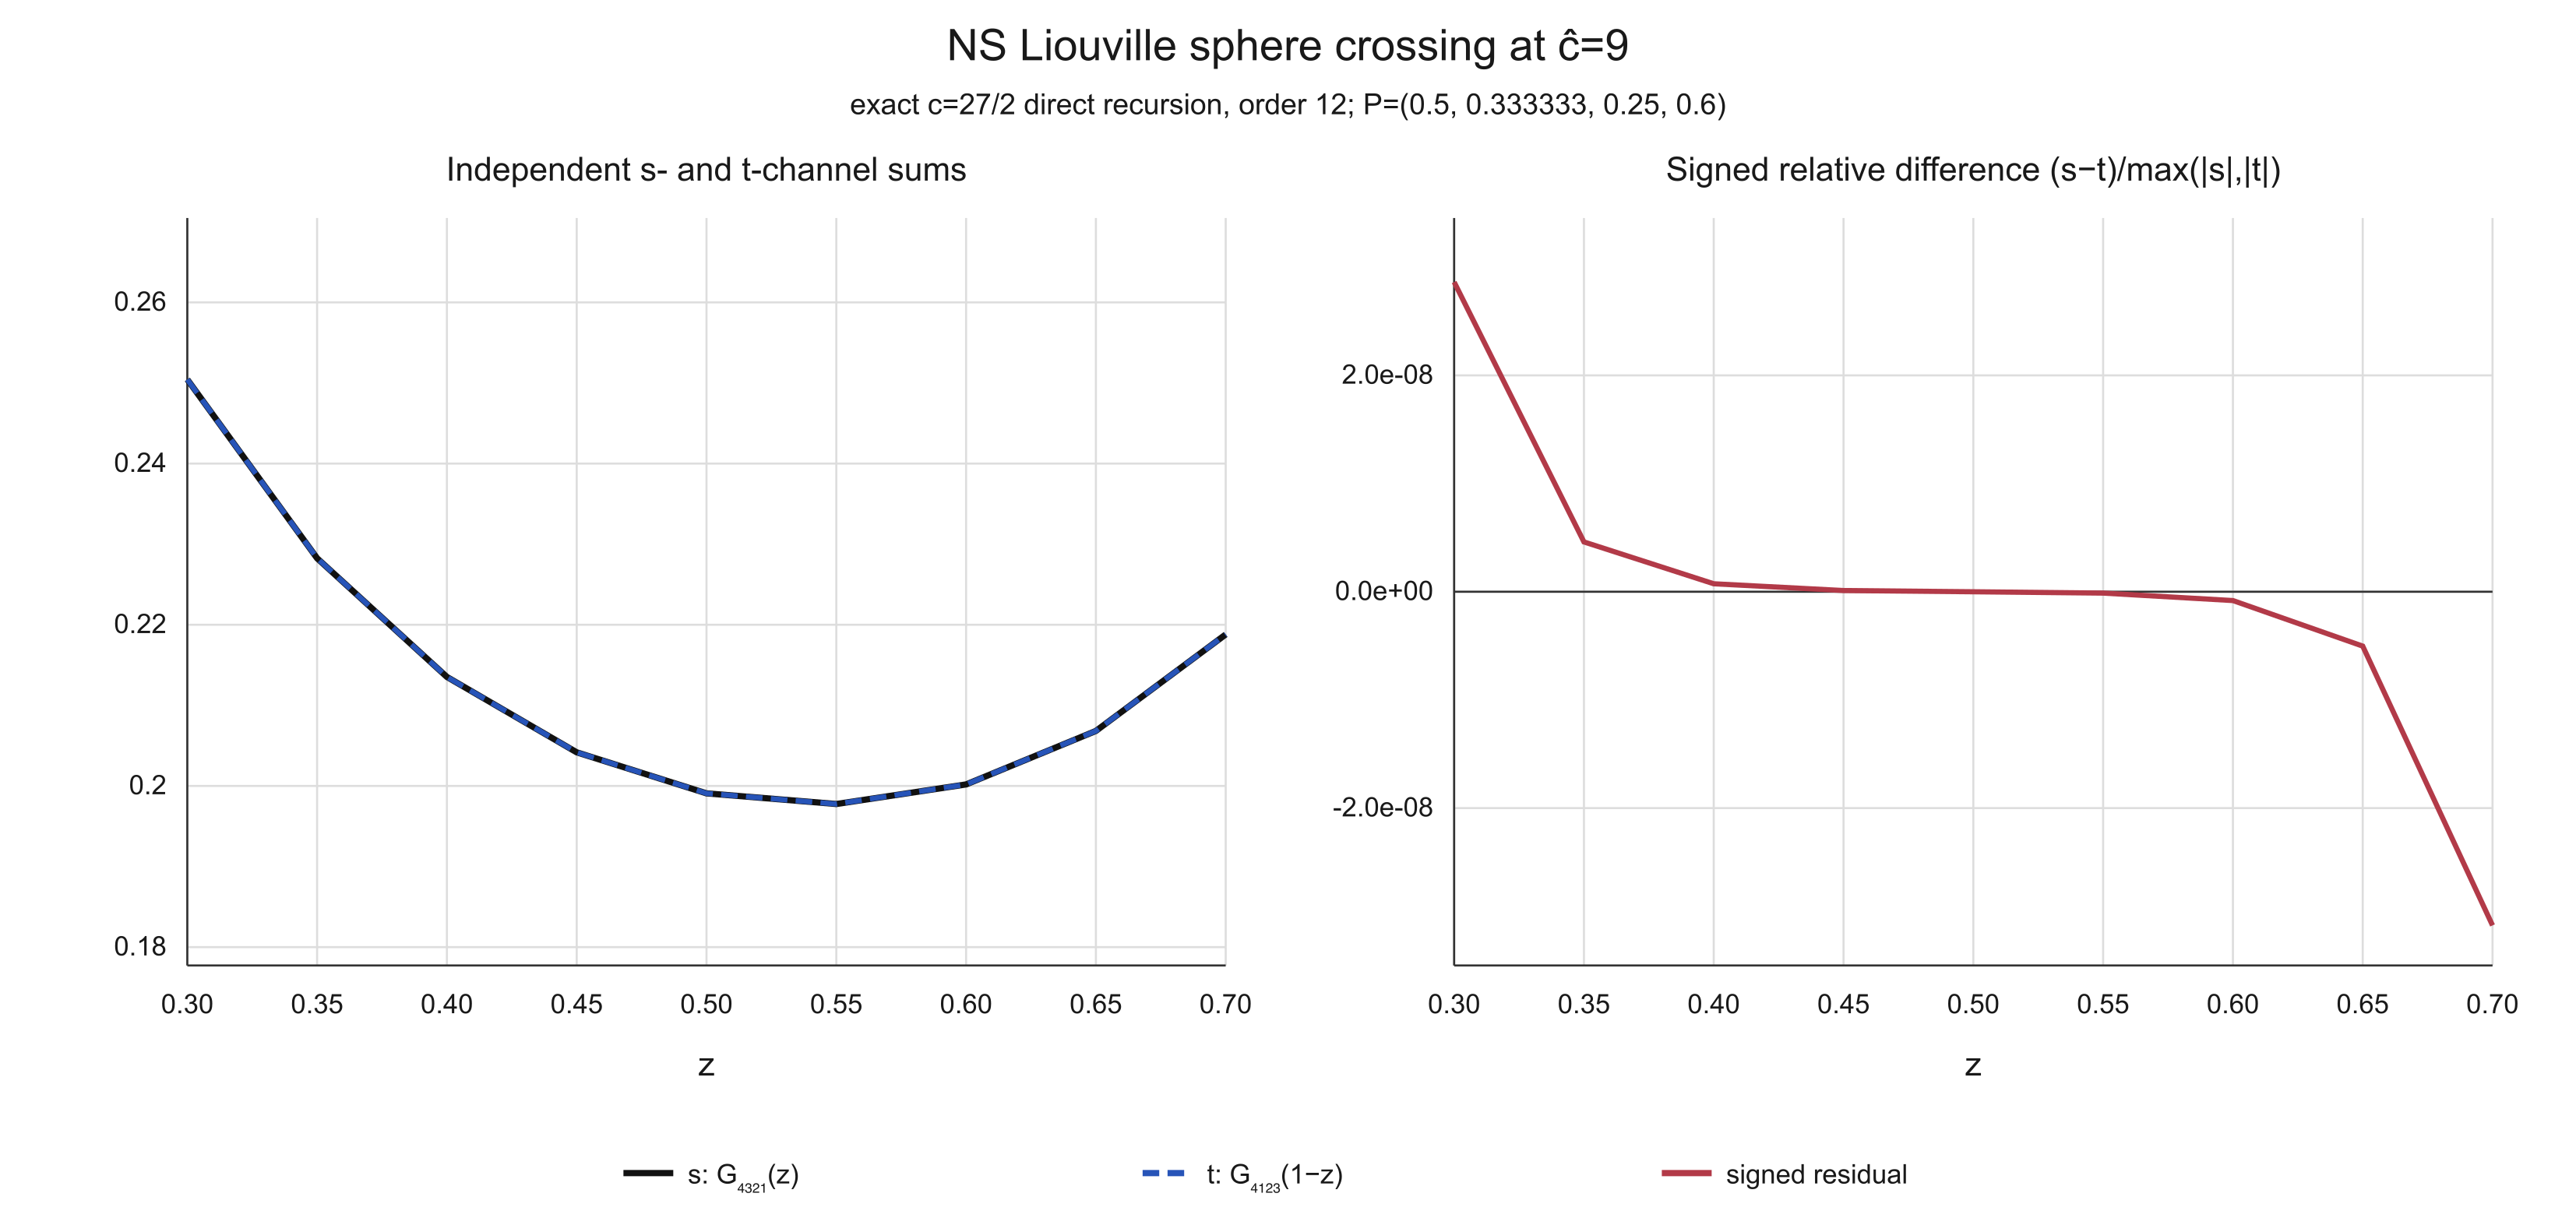
\includegraphics[width=\textwidth]{../../Data Set/ns_liouville_crossing_direct_c_recursion.png}
 \caption{Direct \(c\)-recursion evaluation of the same nonchiral NS
 sphere four-point function in the \(s\)- and \(t\)-channels at
 \(\widehat c=9\).  The right panel shows
 \((G^{(s)}-G^{(t)})/\max(|G^{(s)}|,|G^{(t)}|)\), without assuming
 crossing.}
 \label{fig:ns-sphere-direct-c-crossing}
\end{figure}

The accuracy claim requires a qualification.  At the same 40 momentum nodes,
the maximum order-ten crossing residual is \(3.7697\times10^{-7}\), while
the maximum order-ten to order-twelve drift of either individual channel is
\(3.4612\times10^{-7}\).  The number in
Eq.~\eqref{eq:ns-crossing-order12-result} is therefore an observed
order-twelve residual, not a certified \(3\times10^{-8}\) error bound for the
infinite-recursion correlator.  Increasing the recursion order is postponed.
Moreover, crossing cannot diagnose a systematic error common to both channel
implementations.  The independent \(c\)- versus \(h\)-recursion comparison
above tests the chiral kernel, but the nonchiral structure-constant assembly
and continuum normalization remain shared inputs in this crossing test.

The reproducible implementation, raw ledger, and plot are
\begin{center}
 \path{Code/stress_ns_crossing.py},\\
 \path{Data Set/ns_liouville_crossing_direct_c_recursion_order10.json},\\
 \path{Data Set/ns_liouville_crossing_direct_c_recursion_order12.json},\\
 \path{Data Set/ns_liouville_crossing_direct_c_recursion.svg}.
\end{center}

\subsection{\texorpdfstring{Torus one-point block}
{Torus one-point block}}
\label{sec:torus-one-point-c-h-check}

The torus one-point block provides a second independent comparison with a
known internal-weight recursion.  Closing the single NS edge into a handle,
Eq.~\eqref{eq:master-result} specializes to
\begin{align}
 \F_{1,1}(c,h,d;q,\xi)
 ={}&\U_{1,1}(h,d;q,\xi)\nonumber\\
 &+\sum_{\substack{r\geq2,\ s\geq1\\r+s\in2\mathbb Z}}
 \frac{q^{rs/2}\xi^{rs\bmod2}\,
       \Rcal_{r,s}^{\rm tor}(h,d)}
      {c-c_{r,s}(h)}
 \F_{1,1}\left(c_{r,s}(h),h+\frac{rs}{2},d;q,\xi\right).
 \label{eq:torus-one-point-c-recursion}
\end{align}
The regular term is the product of the non-global NS vacuum character
\eqref{eq:torus-vacuum-character} and the global torus block
\eqref{eq:torus-global}.  The residue contains the two toric null-vector
matrix elements attached to the two ends of the closed edge.  This
fixed-weight \(c\)-recursion was compared with the toric \(h\)-recursion of
Ref.~\cite{HadaszJaskolskiSuchanek2012Toric}.

The comparison concerns the normalized chiral conformal block only.  We set
\begin{equation}
 \rho(\nu_h,\nu_d,\nu_h)=1.
 \label{eq:torus-primary-three-form-normalization}
\end{equation}
No super-Liouville structure constant, reflection amplitude, spectral
measure, or momentum integral is used.  The fusion polynomials in
Eq.~\eqref{eq:torus-one-point-c-recursion} are representation-theoretic
null-vector matrix elements, not dynamical three-point coefficients.

We again used the self-dual point
\begin{equation}
 \widehat c=9,\qquad c=\frac{27}{2},\qquad b=1,
 \qquad
 P_{\rm int}=\frac7{10},\quad h=\frac{149}{200},
 \qquad
 P_{\rm ext}=\frac12,\quad d=\frac58.
 \label{eq:torus-order-ten-benchmark}
\end{equation}
All integer and half-integer powers through \(q^{10}\) were retained.  In
contrast with the sphere plumbing tree, the two values of \(\xi\) are now
the two invariant temporal spin holonomies around the closed torus cycle:
\(\xi=+1\) gives the ordinary NS trace and \(\xi=-1\) inserts
\((-1)^F\).

For the relative discrepancy
\begin{equation}
 \delta_\xi(q)
 =\frac{\left|\F_{1,1}^{(c)}(q,\xi)
                  -\F_{1,1}^{(h)}(q,\xi)\right|}
        {\max\!\left(\left|\F_{1,1}^{(c)}(q,\xi)\right|,
                     \left|\F_{1,1}^{(h)}(q,\xi)\right|\right)},
 \label{eq:torus-c-h-relative-error}
\end{equation}
the ten-point result is
\begin{center}
\scriptsize
\begin{tabular}{@{}rrrrr@{}}
\toprule
\(q\) & \(\F_{\xi=+1}^{(c)}\) & \(\delta_{+}\)
      & \(\F_{\xi=-1}^{(c)}\) & \(\delta_{-}\)\\
\midrule
0.02 & 0.540548101410 & \(3.56\times10^{-64}\)
     & 0.456229368384 & \(3.36\times10^{-64}\)\\
0.04 & 0.647543530569 & \(1.07\times10^{-63}\)
     & 0.505419160552 & \(1.54\times10^{-61}\)\\
0.06 & 0.732306455976 & \(2.10\times10^{-63}\)
     & 0.535126888371 & \(2.04\times10^{-63}\)\\
0.08 & 0.809428769226 & \(3.44\times10^{-63}\)
     & 0.556552964433 & \(3.54\times10^{-63}\)\\
0.10 & 0.884278365341 & \(5.11\times10^{-63}\)
     & 0.573367584001 & \(5.69\times10^{-63}\)\\
0.12 & 0.959753226892 & \(1.62\times10^{-61}\)
     & 0.587248485524 & \(8.75\times10^{-63}\)\\
0.14 & 1.037845659532 & \(9.62\times10^{-63}\)
     & 0.599106998669 & \(1.31\times10^{-62}\)\\
0.16 & 1.120192330357 & \(1.39\times10^{-61}\)
     & 0.609494891429 & \(3.83\times10^{-61}\)\\
0.18 & 1.208326107532 & \(1.71\times10^{-62}\)
     & 0.618772556207 & \(5.04\times10^{-61}\)\\
0.20 & 1.303821014733 & \(2.37\times10^{-62}\)
     & 0.627189301630 & \(6.21\times10^{-61}\)\\
\bottomrule
\end{tabular}
\end{center}
Thus
\begin{equation}
 \max_q\delta_{+}(q)=1.6226\times10^{-61},
 \qquad
 \max_q\delta_{-}(q)=6.2132\times10^{-61}.
 \label{eq:torus-c-h-order-ten-result}
\end{equation}
The coefficient-by-coefficient comparison is equally sharp:
\begin{equation}
 \max_{0\leq n\leq20}
 \frac{|F_{n/2}^{(c)}-F_{n/2}^{(h)}|}
      {\max(|F_{n/2}^{(c)}|,|F_{n/2}^{(h)}|)}
 =5.186\times10^{-58}.
 \label{eq:torus-c-h-coefficient-result}
\end{equation}
The self-dual finite part was extracted at \(60\)-digit working precision
from \(32\) samples on each of the radii \(0.035\) and \(0.045\).  Changing
the radius alters either recursion by at most \(7.35\times10^{-51}\).
At the generic nonresonant point \(b=1.27\), the two recursions agree through
\(q^6\) to \(1.12\times10^{-60}\).  Independent Gram-matrix and Ward-identity
sewing agrees exactly through level one.  The order-ten result is therefore
an agreement of the normalized conformal block, including both torus spin
holonomies, with no theory-dependent OPE data.

The reproducible implementation and numerical ledger are
\begin{center}
 \path{Code/compare_ns_torus_c_h_recursion.py},\\
 \texttt{Machine Notes/c-Recursion/ns\_torus\_c\_h\_order10.json}.
\end{center}

\subsection{Genus-two vacuum theta graph}

Let \(h_1,h_2,h_3\) and \(q_1,q_2,q_3\) label the three edges.  A pole on
edge \(i\) gives
\begin{equation}
 \Rcal_{i;r,s}
 =J_{r,s}(h_i)A_{r,s}(h_i)
  \Sigma_{r,s}^{(L,i)}(h_j,h_k;h_i)
  \Sigma_{r,s}^{(R,i)}(h_j,h_k;h_i),
 \qquad \{i,j,k\}=\{1,2,3\}.
 \label{eq:theta-residue}
\end{equation}
Writing twice-levels as \(\bm\ell,\bm v,\bm r\), the regular term is
\begin{equation}
 \boxed{
 U_{\Theta,\bm\ell}^{\alpha_L,\alpha_R}
 =\sum_{\bm v+\bm r=\bm\ell}
 (-1)^{B_\Theta(\bar{\bm v},\bar{\bm r})}
 V_{\Theta,\bm v}^{(\infty)}
 G_{\Theta,\bm r}^{\osp,\alpha_L,\alpha_R},}
 \label{eq:theta-seed}
\end{equation}
Here \(B_\Theta\) is the six-term polynomial
\eqref{eq:theta-polarized-sign}, the global coefficient is
Eq.~\eqref{eq:global-graph-formula}, and the vacuum coefficients are obtained
by expanding Eq.~\eqref{eq:ns-vacuum-product} with the generators
\eqref{eq:theta-ccy-generators}.  The independently sewn coefficients through
total level six are displayed in Eq.~\eqref{eq:theta-vacuum-level-six}.
Deleting the displayed \((-1)^{B_\Theta}\) gives the wrong answer beginning
at total level \(7/2\); using the correct primitive product gives the same
vacuum coefficients as direct sewing.

\subsubsection{Theta-chart vacuum product}

For a concrete genus-two check, use the theta plumbing coordinates
\(q_0,q_1,q_\infty\).
For edge fermion parities
\(\bm\epsilon=(\epsilon_0,\epsilon_1,\epsilon_\infty)\), the fixed
half-edge ordering used below has
\begin{equation}
 \Omega_\Theta(\bm\epsilon)
 =(-1)^{\epsilon_0\epsilon_1+
        \epsilon_0\epsilon_\infty+
        \epsilon_1\epsilon_\infty+
        \epsilon_\infty}.
 \label{eq:theta-koszul-ledger}
\end{equation}
This is now derived rather than entered by hand.  In vertex-slot order
\((0_L,1_L,\infty_L,0_R,1_R,\infty_R)\), the half-edge frame signs are
\begin{equation}
 ((-1)^{f_h})_{h\in\mathsf H_V}=(+,+,+,+,+,-),
 \qquad (t_0,t_1,t_\infty)=(0,0,0).
 \label{eq:theta-frame-ledger}
\end{equation}
The contraction order \((0_L,0_R,1_L,1_R,\infty_L,\infty_R)\) supplies the
three quadratic inversion terms, while
Eq.~\eqref{eq:frame-derived-beta} gives
\((\beta_0,\beta_1,\beta_\infty)=(0,0,1)\).  Their sum is exactly
Eq.~\eqref{eq:theta-koszul-ledger}.
Consequently an odd null on edge \(e\) carries the coefficient transport
\(\Omega_\Theta(\bm\epsilon)/
  \Omega_\Theta(\bm\epsilon\oplus\ve_e)\).
In the CCY marking, the two projective generators are
\begin{align}
 \gamma_A(z)&=q_0q_\infty z,
 &\gamma_B(z)&=
 \frac{(1-q_1)z-q_0^{-1}}{z-q_0^{-1}}.
 \label{eq:theta-ccy-generators}
\end{align}
The second map depends on \(q_0\), not \(q_\infty\).  Replacing one by the
other preserves the three leading pinching monomials but fails beginning at
the next order.  If \(q_e=t x_e\), the three shortest lifted primitive
classes \(A,B,AB\) have
\begin{align}
 u_A&=\xi_0\xi_\infty(q_0q_\infty)^{1/2},
 \notag\\
 u_B&=-\xi_0\xi_1(q_0q_1)^{1/2}\bigl(1+O(t)\bigr),
 \notag\\
 u_{AB}&=\xi_1\xi_\infty(q_1q_\infty)^{1/2}\bigl(1+O(t)\bigr).
 \label{eq:theta-shortest-lifts}
\end{align}
The middle minus is generated by the determinant-one lift of \(\gamma_B\);
it is not an independently assigned sign.  The three shortest supercurrent
links therefore give
\begin{equation}
\begin{aligned}
 \V_{\Theta,\NS}^{(\infty)}
 ={}&1
 +\xi_0\xi_\infty(q_0q_\infty)^{3/2}
 +\xi_1\xi_\infty(q_1q_\infty)^{3/2}
 -\xi_0\xi_1(q_0q_1)^{3/2}
 +O(t^4).
\end{aligned}
 \label{eq:theta-vacuum-leading}
\end{equation}
Bosonic stress-tensor links begin at order \(t^4\).  The companion Python
implementation computes the exact Schottky multipliers rather than using
these leading expansions.  Expanding that product gives the ordered
CCY-frame vacuum quotient.  Put
\(x_e=\xi_e q_e^{1/2}\).  Direct vacuum Gram-matrix sewing and the
\(c\to\infty\) limit give
\begin{equation}
 \V_{\Theta,\mathrm{pl}}^{(\infty)}
 =1+V_6+V_8+V_{10}+V_{12}+O(|\bm x|^{13}),
 \label{eq:theta-vacuum-level-six}
\end{equation}
where the subscript is total twice-level and
\begin{align}
 V_6={}&x_1^3x_\infty^3+x_0^3x_\infty^3-x_0^3x_1^3,
 \notag\\
 V_8={}&3x_1^3x_\infty^5+x_1^4x_\infty^4+3x_1^5x_\infty^3
 +x_0^4x_\infty^4+x_0^4x_1^4-3x_0^5x_1^3,
 \notag\\
 V_{10}={}&6x_1^3x_\infty^7+4x_1^4x_\infty^6
 +16x_1^5x_\infty^5+4x_1^6x_\infty^4+6x_1^7x_\infty^3
 \notag\\
 &+x_0^5x_\infty^5-x_0^5x_1^5
 +4x_0^6x_1^4-6x_0^7x_1^3,
 \notag\\
 V_{12}={}&10x_1^3x_\infty^9+10x_1^4x_\infty^8
 +50x_1^5x_\infty^7+25x_1^6x_\infty^6
 +50x_1^7x_\infty^5
 \notag\\
 &+10x_1^8x_\infty^4+10x_1^9x_\infty^3
 +x_0^6x_\infty^6+x_0^6x_1^6
 -8x_0^7x_1^5+10x_0^8x_1^4-10x_0^9x_1^3.
 \label{eq:theta-vacuum-level-six-components}
\end{align}
The asymmetry is not a typo: this is the fixed ordered
\((0,1,\infty)\) trinion/BPZ frame.  Equation
\eqref{eq:theta-vacuum-level-six} is independently regenerated in Python by
removing \(G_{-1/2}|0\rangle\) and \(L_{-1}|0\rangle\), sewing the resulting
vacuum quotient, and Richardson-extrapolating in \(1/c\).  It agrees with
the corrected primitive product through every displayed coefficient.

\subsection{Global-block specializations}

\subsubsection{CCY-style sphere six-point block}

The closest comparison with CCY Section 4.3 is the sphere channel with
three internal weights \(h_i\), three plumbing parameters \(q_i\), and
external pairs \((d_1,d_2)\), \((d_3,d_4)\), \((d_5,d_6)\).  For bottom
external components, define the three endpoint factors
\begin{equation}
 E_i(n,\epsilon)
 =\left(h_i+d_{2i}-d_{2i-1}+\frac\epsilon2\right)_n.
 \label{eq:trifundamental-endpoint}
\end{equation}
Let \(\alpha_0\) be the central-trinion sector and \(\alpha_i\) the three
outer sectors.  Then
\begin{equation}
\boxed{
\begin{aligned}
 \G_{6,\rm tri}^{\osp,\bm\alpha}
 ={}&\sum_{\substack{n_i\ge0\\\epsilon_i\in\{0,1\}}}
 \prod_{i=1}^{3}
 \frac{q_i^{n_i+\epsilon_i/2}\xi_i^{\epsilon_i}
       E_i(n_i,\epsilon_i)}
      {n_i!(2h_i)_{n_i+\epsilon_i}}
 \\
 &\times
 \left[\prod_{i=1}^{3}\delta_{\epsilon_i,\alpha_i}\right]
 \delta_{\epsilon_1+\epsilon_2+\epsilon_3
             \equiv\alpha_0\ ({\rm mod}\ 2)}
 T_{n_1,n_2,n_3}^{\epsilon_1\epsilon_2\epsilon_3}
 (h_1,h_2,h_3).
\end{aligned}}
\label{eq:ns-trifundamental-global}
\end{equation}
Up to the displayed parity projectors and the replacement of the central
\(sl(2)\) tensor by Eq.~\eqref{eq:complete-global-vertex}, this is exactly
CCY's Eq.~(4.23).  In particular, setting all \(\epsilon_i=0\) reduces the
central tensor to the CCY three-chain polynomial.

\subsubsection{Sphere four-point global block}

For four bottom components at \(0,z,1,\infty\), fixed even or odd chiral
vertex sectors select \(\epsilon=0\) or \(1\).  Equation
\eqref{eq:global-graph-formula} gives
\begin{equation}
 \G_h^{\osp,(\epsilon)}(z)
 =\sum_{n=0}^{\infty}
 \frac{
  (h+\epsilon/2+h_2-h_1)_n
  (h+\epsilon/2+h_3-h_4)_n}
 {n!\,(2h)_{n+\epsilon}}
 z^{n+\epsilon/2}.
 \label{eq:sphere-global-series}
\end{equation}
Equivalently,
\begin{align}
 \G_h^{\osp,(0)}(z)
 &={}_2F_1(h+h_2-h_1,h+h_3-h_4;2h;z),
 \notag\\
 \G_h^{\osp,(1)}(z)
 &=\frac{z^{1/2}}{2h}
 {}_2F_1\left(h+h_2-h_1+\half,
               h+h_3-h_4+\half;
               2h+1;z\right).
 \label{eq:sphere-global-hypergeometric}
\end{align}
Their lift-refined direct sum is
\(\G_h^{\osp,(0)}+\xi\G_h^{\osp,(1)}\).  It is the light block in the
component-normalized convention of Ref.~\cite{BelavinGeiko2018CRecursion},
whereas fixed parity-homogeneous three-forms use one summand.  This is the
four-point instance of Eq.~\eqref{eq:vertex-parity-projector}.

\subsubsection{Torus one-point global block}

For one internal edge closed into a handle and a bottom primary insertion of
weight \(d\), both ends of the edge carry the same \(\epsilon\), so the
even trinion structure admits both integer and half-integer levels:
\begin{equation}
 \G_{1,1}^{\osp,(0)}(h,d;q,\xi)
 =\sum_{n\ge0}\sum_{\epsilon=0}^{1}
 \frac{q^{n+\epsilon/2}\xi^\epsilon\,
 T_{n,0,n}^{\epsilon,0,\epsilon}(h,d,h)}
 {n!(2h)_{n+\epsilon}}.
 \label{eq:torus-global}
\end{equation}
The first terms are
\begin{equation}
 \G_{1,1}^{\osp,(0)}
 =1+\xi q^{1/2}\frac{2h-d}{2h}
   +q\frac{2h+d(d-1)}{2h}+O(q^{3/2}),
 \label{eq:torus-global-first-terms}
\end{equation}
in agreement with the direct super-Virasoro computation of
Ref.~\cite{BelavinGeiko2018CRecursion}.


\subsection{Coefficient implementation}
\label{sec:computational-graded-factorization}

At a fixed cutoff, store the vacuum and global series as dictionaries
indexed by twice-level vectors,
\begin{equation}
 V=\sum_{\bm v}V_{\bm v}\bm q^{\bm v/2},
 \qquad
 G=\sum_{\bm r}G_{\bm r}\bm q^{\bm r/2}.
 \label{eq:series-dictionaries}
\end{equation}
Ordinary multiplication of the already oriented scalar series would omit the
polarized sign.  The explicit theta-plumbing loop is
\begin{verbatim}
for vacuum_level, vacuum_coefficient in vacuum.items():
    global_level = level - vacuum_level
    if min(global_level) < 0:
        continue
    vacuum_parity = tuple(n % 2 for n in vacuum_level)
    global_parity = tuple(n % 2 for n in global_level)
    cross_sign = orientation.cross_sign(
        vacuum_parity, global_parity
    )
    regular[level] += (
        cross_sign * vacuum_coefficient * global[global_level]
    )
\end{verbatim}
Here \verb|orientation.cross_sign| evaluates the inversion sum
\eqref{eq:graph-orientation-polarization}; its implementation is
\path{Code/ns_regular_block.py}.
The lift monomial attached to this summand is
\(\prod_e\xi_e^{v_e\bmod2}\xi_e^{r_e\bmod2}\), which equals the lift
monomial at \(\bm\ell=\bm v+\bm r\).

For example, take
\begin{equation}
 \bm\ell=(0,3,4),\qquad
 \bm v=(0,3,3),\qquad
 \bm r=(0,0,1).
 \label{eq:graded-convolution-example-levels}
\end{equation}
Their parity vectors give
\begin{equation}
 \Omega_\Theta(\bm\ell)=+1,\qquad
 \Omega_\Theta(\bm v)=+1,\qquad
 \Omega_\Theta(\bm r)=-1,
 \label{eq:graded-convolution-example-signs}
\end{equation}
so Eq.~\eqref{eq:theta-polarized-sign} gives \(B_\Theta=1\) and the cross
sign is \(-1\).  At the benchmark point
\eqref{eq:finite-c-benchmark-point},
\begin{equation}
 V_{(0,3,3)}=1,\qquad
 G_{(0,0,1)}=-0.427350427350427\ldots,
\end{equation}
and this splitting contributes
\(+0.427350427350427\ldots\).  The opposite sign from naive multiplication
is therefore traced to one explicit half-edge inversion.

The left-hand side of the finite-\(c\) check is constructed without any
recursion.  If \(\mathcal B_e(\ell_e)\) is the NS PBW basis and
\(B_e^{(\ell_e)}\) its Gram matrix, the direct theta coefficient is
\begin{equation}
 D_{\bm\ell}(c)
 =\Omega_\Theta(\bm\ell)
  \prod_e\xi_e^{\ell_e\bmod2}
  \rho_{abc}
  (B_0^{-1})^{aa'}(B_1^{-1})^{bb'}
  (B_\infty^{-1})^{cc'}
  \rho_{a'b'c'}.
 \label{eq:direct-theta-computational-contraction}
\end{equation}
The code generates the three PBW bases, normal-orders the super-Virasoro
algebra to form the Gram matrices, evaluates every entry of \(\rho\) from the
NS Ward identities, and performs the displayed tensor contraction.

The regular input is computed independently.  For the vacuum part, delete
all PBW words containing \(G_{-1/2}\) or \(L_{-1}\), sew the resulting
irreducible vacuum bases by the same operation
\eqref{eq:direct-theta-computational-contraction}, and evaluate at five large
generic central charges \(c_j\).  At every level the values are fitted as
\begin{equation}
 D^{\rm vac}_{\bm v}(c_j)
 =V_{\bm v}+\frac{a_1}{c_j}+\frac{a_2}{c_j^2}+\cdots,
 \label{eq:vacuum-richardson-extraction}
\end{equation}
so the constant term gives the CCY-frame vacuum coefficient.  This vacuum
calculation has no generic internal weights and uses no Kac residues.  It is
then combined with the closed global coefficient by
Eq.~\eqref{eq:regular-coefficient-formula} to obtain \(U_{\bm\ell}\).

Finally, the program adds every admissible local Kac residue with
\(rs\le2\ell_e\).  It lowers the twice-level on edge \(e\) by \(rs\), shifts
\(h_e\) by \(rs/2\), toggles both adjacent vertex sectors when \(rs\) is odd,
and applies the null-level lift and orientation-transport signs.  The result
is compared coefficient by coefficient with \(D_{\bm\ell}(c)\).  At total
level six the integer triples obey
\begin{equation}
 n_0+n_1+n_\infty\le12,qquad n_e=2\ell_e,
\end{equation}
and hence there are
\begin{equation}
 \#\{\bm n\}=\binom{12+3}{3}=455
 \label{eq:level-six-coefficient-count}
\end{equation}
independent coefficient comparisons.

Belavin--Geiko establish the sphere and torus versions explicitly
\cite{BelavinGeiko2018CRecursion}.  Nothing in the counting uses a special
graph: it applies independently at every trinion and every inverse metric.


\subsection{Automated checks}
\label{sec:python-checks}

The general recursion checks are implemented in
\begin{center}
 \path{Code/ns_genus_c_recursion_checks.py}
\end{center}
and are deliberately small and representation-theoretic.  The script can be
run from the
repository root as
\begin{verbatim}
python3 Code/ns_genus_c_recursion_checks.py
\end{verbatim}
or with \verb|--json|.  It performs the following independent checks.
\begin{enumerate}
 \item It substitutes \(b_{3,1}(h)\) into
 \(h_{3,1}(c(b))\) and checks the pole equation.
 \item It compares Eq.~\eqref{eq:jacobian-explicit} with a centered finite
 difference of \(c_{3,1}(h)\).
 \item It evaluates Eq.~\eqref{eq:global-norm} and the sphere coefficients
 \eqref{eq:sphere-global-series}, then compares them through twice-level
 eight with the production NS sphere seed in
 \path{Code/superconformal_blocks.py}.
 \item It inverts Eq.~\eqref{eq:level-three-half-gram} at
 \(c=10^3\) and \(10^6\) and verifies suppression of the non-global
 state.
 \item It constructs Eq.~\eqref{eq:torus-vacuum-character} by a product
 recursion and independently by explicit bosonic occupation/fermionic subset
 enumeration, for both lift signs.
\end{enumerate}
The global calculation is implemented separately in
\begin{center}
 \path{Code/ns_global_osp_block.py}.
\end{center}
It implements the six independent kernels in
Eq.~\eqref{eq:eight-global-kernels}, the two reflected kernels in
Eq.~\eqref{eq:projected-global-reflection}, the
three-chain completion \eqref{eq:complete-global-vertex}, the parity
projector, and the trifundamental coefficient
\eqref{eq:ns-trifundamental-global}.  Its checks use
Eq.~\eqref{eq:global-raising}, the endpoint reduction
\eqref{eq:trifundamental-endpoint}, the zero-level Ward table, the CCY
middle-chain identity \eqref{eq:ccy-middle-chain-limit}, and the two
published torus coefficients \eqref{eq:torus-global-first-terms}.

The independent superspace derivation is implemented in
\begin{center}
 \path{Code/ns_osp_superspace.py}.
\end{center}
It first expands \(Z_{ij}\) and \(\eta_{123}\) in a symbolic three-generator
exterior algebra and verifies that the result is exactly
Eq.~\eqref{eq:compact-superspace-component-kernel}.  It then differentiates
that kernel according to Eq.~\eqref{eq:compact-derivative-global-vertex} and
compares against \path{Code/ns_global_osp_block.py}.  The check covers all
eight Grassmann sectors and all triples of occupations through three on two
generic rational weight assignments; all \(1024\) descendant coefficients
agree.

The genuine-supermoduli plumbing check is implemented in
\begin{center}
 \path{Code/ns_supermoduli_plumbing.py}.
\end{center}
It verifies \(\mathscr D^2=\partial\), checks that the even edge count and
odd vertex count reproduce Eq.~\eqref{eq:ns-supermoduli-dimension}, and
constructs the two-vertex sphere generating block explicitly.  Ordered
integration over its two vertex moduli reproduces \(256\) directly sewn
sector coefficients through bosonic occupation three with zero error.

The independent exterior-algebra implementation
\begin{center}
 \path{Code/ns_grassmann_sewing.py}
\end{center}
constructs the edge kernel \eqref{eq:osp-berezin-edge-kernel}, performs the
ordered Berezin integral, and compares it with the component contraction.  It
checks all eight theta-graph parity assignments, a punctured orientation with
both external parities, and the even/odd inverse-Gram normalization
\eqref{eq:berezin-even-odd-norms}.

The lifted Schottky calculation is implemented in
\begin{center}
 \path{Code/ns_vacuum_schottky.py}.
\end{center}
It enumerates primitive cyclic words modulo inversion, constructs the chosen
\(SL(2)\) lift of each word, extracts \((u_\gamma,k_\gamma)\), and evaluates
Eq.~\eqref{eq:ns-vacuum-product}.  Its tests are independent at the relevant
steps:
\begin{enumerate}
 \item compare \(u_\gamma^2\) with the projective multiplier for all
 primitive words through length five and verify cyclic/inverse invariance;
 \item compare the genus-one Schottky evaluation with a direct oscillator
 product for both lift signs;
 \item test the exterior-Fock trace-log identity
 \eqref{eq:exterior-fock-determinant} on a finite complex kernel;
 \item compare the bosonic denominator exactly with the existing CCY
 implementation in \path{Code/python/genus2_vacuum_blocks.py};
 \item scale the theta plumbing parameters uniformly and verify convergence
 to the three-link coefficient \eqref{eq:theta-vacuum-leading} for all eight
 edge-lift assignments;
 \item subtract the entire independently sewn vacuum table through total
 level six for all eight lift assignments.  Under \(q_e\mapsto q_e/2\), the
 maximum remainder ratio is \(0.00647\), consistent with a first omitted
 contribution at total level seven and incompatible with a mismatch at level
 six or below.
\end{enumerate}

The half-edge sign calculation is implemented in
\begin{center}
 \path{Code/ns_regular_block.py}.
\end{center}
Given the ordered pairs of internal half-edges and the contraction
permutation, it evaluates \(Q_\Gamma\) by inversion counting, checks that its
linear BPZ part drops out of the polarization, and evaluates
Eq.~\eqref{eq:regular-coefficient-formula}.  For the theta graph it
regenerates both Eqs.~\eqref{eq:theta-koszul-ledger} and
\eqref{eq:theta-polarized-sign}.

The direct finite-\(c\) comparison is implemented in
\begin{center}
 \path{Code/ns_genus12_finite_c_check.py}.
\end{center}
It does not call the recursion to construct its left-hand side.  It
enumerates the NS PBW basis, normal-orders the super-Virasoro algebra to
obtain every Gram matrix, evaluates the full three-descendant tensor from
the NS Ward identities, inverts the three edge Gram matrices, and contracts
the two theta-graph trinions.  The genus-two cutoff is total plumbing level,
the same convention as the repository's CCY bosonic checker.
For the regular term it separately constructs the irreducible vacuum basis
by deleting every PBW word containing \(G_{-1/2}\) or \(L_{-1}\), computes
the vacuum Gram matrices and Ward tensors, and takes the large-\(c\) limit by
a five-point Richardson extrapolation in \(1/c\).  It combines this table
with the global coefficients using the explicit polarization routine, not a
named product.  Hence the vacuum table is not fitted from the generic
finite-\(c\) block used on the left-hand side.

For the reproducible generic point
\begin{equation}
 c=37.25,\qquad (h_0,h_1,h_\infty)=(0.73,0.91,1.17),
 \qquad (\xi_0,\xi_1,\xi_\infty)=(1,1,1),
 \label{eq:finite-c-benchmark-point}
\end{equation}
the genus-one trace gives, through level \(6\),
\begin{equation}
 1+\xi q^{1/2}+q+2\xi q^{3/2}+3q^2+4\xi q^{5/2}
 +5q^3+7\xi q^{7/2}+10q^4+13\xi q^{9/2}
 +16q^5+21\xi q^{11/2}+28q^6.
 \label{eq:genus-one-direct-level-four}
\end{equation}
This equals the generic NS character exactly: at each level the direct
contraction is \(\operatorname{Tr}(B^{-1}B)\), so there is no residual
\(c\)-dependence.

At genus two the script compares every triple
\((\ell_0,\ell_1,\ell_\infty)\) with
\(\ell_0+\ell_1+\ell_\infty\le6\): \(455\) coefficients in total.  Some
representative values are
\begin{center}
\begin{tabular}{@{}c r r r@{}}
\toprule
\(2\bm\ell\) & regular \(U_{\bm\ell}\) & direct finite \(c\)
& recursion\\
\midrule
\((3,0,0)\) & \(0.261972379997773\) & \(0.263840424020828\)
& \(0.263840424020828\)\\
\((0,0,3)\) & \(-0.437906238804443\) & \(-0.438382932952886\)
& \(-0.438382932952887\)\\
\((1,0,4)\) & \(0.108351800526099\) & \(0.175068774562786\)
& \(0.175068774562786\)\\
\((3,3,0)\) & \(-1.00317218140405\) & \(-1.04112826090143\)
& \(-1.04112826090143\)\\
\((3,0,3)\) & \(1.24049898969217\) & \(1.12019936770983\)
& \(1.12019936770983\)\\
\((0,3,3)\) & \(3.81585349350960\) & \(3.95674683480596\)
& \(3.95674683480596\)\\
\((0,4,2)\) & \(4.70247533416103\) & \(4.87540464672133\)
& \(4.87540464672133\)\\
\((0,0,6)\) & \(0.554995640172376\) & \(0.618077510729804\)
& \(0.618077510729803\)\\
\bottomrule
\end{tabular}
\end{center}
The maximum direct-versus-recursive error at each total twice-level
\(0,1,\ldots,12\) is
\begin{equation}
 \begin{aligned}
 (&0,\ 0,\ 1.39{\times}10^{-16},\ 2.22{\times}10^{-16},\
  3.33{\times}10^{-16},\\
 &7.77{\times}10^{-16},\ 8.88{\times}10^{-16},\
  2.66{\times}10^{-15},\ 7.99{\times}10^{-15},\\
 &1.42{\times}10^{-14},\ 2.84{\times}10^{-14},\
  4.26{\times}10^{-14},\ 5.36{\times}10^{-13}).
 \end{aligned}
 \label{eq:genus-two-error-by-level}
\end{equation}
The worst coefficient is \(2\bm\ell=(0,1,11)\).  Two additional generic
benchmark points give maximum errors \(1.28\times10^{-12}\) and
\(8.70\times10^{-14}\).  The independent vacuum-quotient extraction agrees
with the integer table \eqref{eq:theta-vacuum-level-six-components} to
\(1.24\times10^{-14}\).

This higher cutoff is also a falsification test.  Keeping the correct vacuum
coefficients but deleting the polarized sign in
Eq.~\eqref{eq:theta-seed} gives an error \(1.37\) already at
\(2\bm\ell=(4,0,3)\).  Thus the level-three pass could not have detected the
missing cross sign, because the first vacuum terms there only multiply the
constant global coefficient.

The current output of all five scripts includes
\begin{center}
\begin{tabular}{@{}L{0.67\textwidth}l@{}}
\toprule
Check & Result\\
\midrule
Kac pole equation error & \(3.33\times10^{-16}\)\\
Jacobian relative error & \(1.50\times10^{-10}\)\\
Maximum sphere global-seed error & \(0\)\\
Level-\(3/2\) non-global error at \(c=10^3\) & \(1.14\times10^{-3}\)\\
Level-\(3/2\) non-global error at \(c=10^6\) & \(1.14\times10^{-6}\)\\
Vacuum product versus Fock enumeration & pass\\
Global norm recursion maximum error & \(7.11\times10^{-15}\)\\
Endpoint and primary Ward-table errors & \(0\)\\
CCY middle-chain identity error & \(3.55\times10^{-14}\)\\
Torus levels \(1/2\) and \(1\) errors
& \(0,\ 3.33\times10^{-16}\)\\
Trinion parity projector & pass\\
Lift relation \(u_\gamma^2=k_\gamma\), maximum relative error
& \(9.95\times10^{-16}\)\\
Cyclic/inverse half-multiplier error & \(4.58\times10^{-16}\)\\
Lifted genus-one product error & \(2.22\times10^{-16}\)\\
Exterior trace-log error & \(0\)\\
Bosonic reduction versus CCY & \(0\)\\
Theta leading-error ratio under \(t\mapsto t/2\) & \(0.489\)\\
Corrected primitive product versus the level-six vacuum table:
remainder ratio under \(t\mapsto t/2\) & \(0.00647<2^{-7}\)\\
General half-edge polarization algorithm & pass\\
Vacuum quotient versus level-six seed & \(1.24\times10^{-14}\) maximum\\
Genus-one direct versus recursion through level \(6\) & exact\\
Genus-two direct versus recursion, \(455\) coefficients
& \(5.36\times10^{-13}\) maximum\\
\bottomrule
\end{tabular}
\end{center}
These checks certify the pole data, the global factor, the direct CCY-frame
vacuum seed, and the assembled finite-\(c\) recursion through total level six.
The corrected product remainder scales as level seven after subtracting the
entire level-six direct table, so it excludes a product/sewing mismatch at
any displayed level.  The all-order identification itself follows from the
primitive-link derivation, rather than from this finite truncation.

\subsection{\texorpdfstring{Direct finite-\(c\) stress tests}
{Direct finite-c stress tests}}
\label{sec:coefficient-stress-tests}

The preceding checks test the ingredients of the construction separately.
We also performed a direct coefficient-by-coefficient comparison of the
assembled recursion with the finite-level block.  This is the cleanest
test of the recursion formula itself.  Write
\begin{equation}
 D_{\bm n}(c,\bm h)
 \quad\hbox{and}\quad
 R_{\bm n}(c,\bm h),
 \qquad \bm n=(n_0,n_1,n_\infty)=2\bm\ell,
 \label{eq:direct-recursive-coefficients}
\end{equation}
for, respectively, the coefficient obtained by direct PBW sewing and the
coefficient obtained by expanding the recursion relation to the same
twice-level.  No numerical power-series extrapolation is involved: at a
fixed cutoff both constructions produce the coefficient itself.  Possible
floating-point error enters only if the resulting rational functions are
subsequently evaluated numerically.

\subsubsection{Exact symbolic comparison through total order three}

The script \path{Code/ns_genus2_symbolic_low_order.py} carries out the two
constructions independently over
\(\mathbb Q(c,h_0,h_1,h_\infty)\).  Direct Gram-matrix inversion and Ward
contractions are used on one side, whereas the global seed, Kac residues,
weight shifts, and edge-orientation signs are assembled on the other.  For
all
\begin{equation}
 n_0+n_1+n_\infty\leq 6,
 \label{eq:symbolic-check-range}
\end{equation}
the script simplifies \(D_{\bm n}-R_{\bm n}\) as an exact rational
function.  Thus this range contains all \(84=\binom{9}{3}\) coefficients
through total physical order three, rather than a sample of coefficients.

The relevant degenerate central charges in this range are
\begin{align}
 c_{3,1}(h)&=6-3h-\frac{6}{2h+1}
            =-\frac{3h(2h-3)}{2h+1},\nonumber\\
 c_{2,2}(h)&=\frac32-8h,\nonumber\\
 c_{5,1}(h)&=\frac{13}{2}-h-\frac{9}{h+1}
            =-\frac{(h-5)(2h-1)}{2(h+1)}.
 \label{eq:symbolic-low-order-poles}
\end{align}
Representative identities expose more than agreement of two final
numbers.  Define
\begin{equation}
 \Delta_0=(2h_0+1)c+6h_0^2-9h_0
          =(2h_0+1)\bigl(c-c_{3,1}(h_0)\bigr).
 \label{eq:symbolic-delta-zero}
\end{equation}
At twice-level \((3,0,0)\), direct sewing gives
\begin{align}
 U_{300}
 &=\frac{(2h_0+2h_1-2h_\infty+1)^2}
         {8h_0(2h_0+1)},\nonumber\\
 D_{300}-U_{300}
 &=\frac{6(h_1-h_\infty)^2}{(2h_0+1)\Delta_0}
  =\frac{1}{c-c_{3,1}(h_0)}
    \frac{6(h_1-h_\infty)^2}{(2h_0+1)^2}.
 \label{eq:symbolic-300-check}
\end{align}
The first term is the global coefficient and the second is exactly the
\((3,1)\) odd residue prescribed by the recursion.

The mixed coefficient \((3,1,0)\) checks both the shifted block and the
orientation sign.  With
\begin{equation}
 \mathcal A=2h_0h_1+2h_0h_\infty-h_0-2h_1^2
 +4h_1h_\infty+h_1-2h_\infty^2+h_\infty,
 \label{eq:symbolic-A-polynomial}
\end{equation}
one finds
\begin{equation}
 D_{310}-U_{310}
 =-\frac{3\mathcal A^2}{4h_1(2h_0+1)\Delta_0}
 =-\frac{1}{c-c_{3,1}(h_0)}
   \frac{3\mathcal A^2}{2(2h_0+1)^2}\,
   \frac{1}{2h_1}.
 \label{eq:symbolic-310-check}
\end{equation}
Here \(1/(2h_1)\) is the shifted global coefficient and the minus sign is
the theta-graph orientation transport.  At twice-level \((4,0,0)\), the
same comparison resolves the two distinct pole channels separately:
\begin{equation}
 D_{400}=U_{400}
 +\frac{R^{\mathrm{even}}_{3,1}(h_0)}
        {c-c_{3,1}(h_0)}\frac{1}{2h_0+3}
 +\frac{R^{\mathrm{even}}_{2,2}(h_0)}
        {c-c_{2,2}(h_0)},
 \label{eq:symbolic-400-check}
\end{equation}
where
\begin{align}
 R^{\mathrm{even}}_{3,1}(h_0)
 &=\frac{3\mathcal A^2}{2(2h_0+1)^2},\nonumber\\
 R^{\mathrm{even}}_{2,2}(h_0)
 &=\frac{\mathcal B^2}{4h_0(2h_0+3)},\nonumber\\
 \mathcal B&=h_0^2+2h_0h_1+2h_0h_\infty
 -3h_1^2+6h_1h_\infty-3h_\infty^2.
 \label{eq:symbolic-even-residues}
\end{align}
The identities at \((5,0,0)\), \((3,3,0)\), and \((6,0,0)\) additionally
exercise the \((5,1)\) channel, simultaneous edge contributions, and all
channels available at the cutoff; each simplifies identically to zero.
Altogether the exact result is
\begin{equation}
 D_{\bm n}-R_{\bm n}=0
 \qquad\text{for all }\bm n\in\mathbb Z_{\geq0}^3,
 \quad |\bm n|\leq6,
 \qquad 84/84\ \text{identities}.
 \label{eq:symbolic-84-result}
\end{equation}

The same calculation fixes the first nontrivial theta-graph vacuum seed
directly from the large-\(c\) limit:
\begin{equation}
 \lim_{c\to\infty}(D_{033}-G_{033})=1,
 \qquad
 \lim_{c\to\infty}(D_{303}-G_{303})=1,
 \qquad
 \lim_{c\to\infty}(D_{330}-G_{330})=-1.
 \label{eq:exact-first-vacuum-seed}
\end{equation}
This verifies the relative sign in the first theta contribution without
using the Schottky product as input.  As a secondary check, evaluating all
84 symbolic answers at an independent generic point agrees with the direct
and recursive numerical implementations to \(1.78\times10^{-15}\) and
\(3.11\times10^{-15}\), respectively.

\subsubsection{Finite-level stress test through total order eight}

The independent finite-level implementation
\path{Code/ns_genus12_finite_c_check.py} was then used at larger cutoffs.
First, the previously reported order-six test was rerun without modifying
its conventions or benchmark.  All
\(455=\binom{15}{3}\) coefficients with
\(n_0+n_1+n_\infty\leq12\) agree, with maximum absolute discrepancy
\(5.36\times10^{-13}\).  The earlier order-six check is therefore faithful.

For the order-eight test we chose the generic point
\begin{equation}
 c=41.3,
 \qquad (h_0,h_1,h_\infty)=(0.731,0.913,1.173),
 \qquad (\xi_0,\xi_1,\xi_\infty)=(1,1,1).
 \label{eq:order-eight-benchmark}
\end{equation}
All \(969=\binom{19}{3}\) coefficients with
\(n_0+n_1+n_\infty\leq16\) pass.  The largest absolute discrepancy is
\(1.071\times10^{-9}\), at \((0,5,11)\), where the two values are
\begin{equation}
 767.8733692113085
 \qquad\hbox{and}\qquad
 767.8733692123799.
 \label{eq:order-eight-largest-error}
\end{equation}
After division by the natural coefficient scale, the largest discrepancy
over the full table is \(9.124\times10^{-11}\).  These residuals are solely
from floating-point evaluation of Gram inverses, residues, and shifted
blocks; the comparison is between coefficients at a fixed cutoff and hence
has no truncation remainder.

Two vacuum checks accompany the finite-\(c\) comparison.  Direct large-\(c\)
extraction through order eight produces \(97\) nonzero integer vacuum-seed
coefficients, with maximum numerical extraction error
\(2.84\times10^{-13}\).  Subtracting the complete order-eight table from the
corrected primitive Schottky product gives a remainder ratio
\begin{equation}
 \frac{|\mathcal E(t/2)|}{|\mathcal E(t)|}=0.002881861
 \qquad (t=0.08),
 \label{eq:order-eight-schottky-remainder}
\end{equation}
uniformly for all eight choices of the three edge lifts.  This is compatible
with the first omitted terms beginning at total order nine, at the finite
values of \(t\) used in the test.

The higher-order run also exposed a useful exceptional-point issue.  The
old order-six benchmark remains generic throughout its tested range, but at
higher shifted levels it encounters a coincident pole: at top twice-level
\((10,3,0)\) and \(c=1.1423404255\ldots\), the shifted \((5,1)\) pole on edge
zero coincides with the shifted \((3,1)\) pole on edge one.  The formal
recursion then requires weight detuning or a higher-order Laurent recursion;
the scalar numerical evaluator now reports this unsupported collision
explicitly.  The exact double pole in Eq.~\eqref{eq:d330-double-pole} shows
why merging equal simple-pole keys would not suffice.
This is not a disagreement of generic coefficients, but it explains why a
benchmark that is safe through order six need not remain safe at order
eight.

In summary, on the generic locus the recursion has passed an exact symbolic
comparison of every coefficient through total order three and an independent
numerical stress test of every coefficient through total order eight.  These
tests strongly support the order-by-order prescription, including its residue
channels, shifted sub-blocks, lift signs, and vacuum seed in the theta-graph
orientation convention.  The sign compiler above reconstructs that
convention from its half-edge frames and transition lifts, including
\((\beta_0,\beta_1,\beta_\infty)=(0,0,1)\).  The tests do not implement
exceptional higher-order poles.


\subsection{Companion code}

The formulas are implemented in a small set of independent scripts:
\begin{center}
\small
\begin{tabularx}{\textwidth}{@{}L{0.49\textwidth}X@{}}
\toprule
Script & Role\\
\midrule
\path{Code/superconformal_blocks.py} & sphere NS \(c\)-recursion kernel\\
\path{Code/superconformal_torus_blocks.py} & toric NS \(h\)-recursion and spin-lifted evaluation\\
\path{Code/ns_global_osp_block.py} & component global module and trinion kernels\\
\path{Code/ns_regular_block.py} & endpoint reflection/Koszul signs, frame-derived orientation, polarization, and regular-block assembly\\
\path{Code/ns_vacuum_schottky.py} & lifted primitive Schottky product\\
\path{Code/compare_ns_sphere_c_h_recursion.py} & order-ten sphere \(c\)- versus \(h\)-recursion comparison at \(\widehat c=9\)\\
\path{Code/stress_ns_crossing.py} & direct-recursion nonchiral sphere crossing test at \(\widehat c=9\)\\
\path{Code/compare_ns_torus_c_h_recursion.py} & order-ten torus one-point \(c\)- versus \(h\)-recursion comparison at \(\widehat c=9\)\\
\path{Code/ns_genus12_finite_c_check.py} & direct genus-one and genus-two finite-\(c\) sewing\\
\path{Code/ns_genus2_symbolic_low_order.py} & exact symbolic coefficient comparison\\
\path{Code/ns_osp_superspace.py}, \path{Code/ns_supermoduli_plumbing.py} & optional superspace and supermoduli reformulations\\
\bottomrule
\end{tabularx}
\end{center}

\section*{Conclusion}
\addcontentsline{toc}{section}{Conclusion}

The NS \(c\)-recursion has two independent ingredients.  Representation
theory fixes every moving pole and its edge-local residue.  The CCY
large-\(c\) separation fixes the regular term as the graded assembly of the
explicit global \(\osp\) network and the universal lifted vacuum product.
Together they give the functional recursion
\eqref{eq:master-result} and its triangular coefficient form
\eqref{eq:coefficient-recursion} at generic weights for an arbitrary ordered
plumbing graph.  Equations~\eqref{eq:canonical-endpoint-sign} and
\eqref{eq:frame-derived-beta} compute the endpoint and BPZ/spin-frame signs
from the ordered lifted local coordinates, so no independent sign table is
left unspecified.  The present manuscript does not extend the recursion to
coincident Kac loci.

The genus-\(g\), zero-point block is the literal \(N=0\) specialization
\eqref{eq:genus-g-zero-point-regular}; in the irreducible vacuum channel it
reduces to the primitive product \eqref{eq:genus-g-vacuum-regular}.  Direct
PBW sewing confirms the assembled recursion at genus one and genus two
through the cutoffs recorded in Section~\ref{sec:consistency-checks}.
Superspace provides a compact reformulation, but no step of the main
derivation depends on the exploratory odd-moduli plumbing proposal.

\bibliographystyle{unsrt}
\bibliography{../../References/references}

\end{document}
